% =====================================================================================
%  GIM v20.1.0 -- model description manuscript
%  Target: Geoscientific Model Development (model description paper)
%
%  COMPILING ON OVERLEAF
%  ---------------------
%  Compiler: pdfLaTeX (Menu -> Compiler -> pdfLaTeX).  Run: pdflatex -> bibtex -> pdflatex x2.
%  This file is deliberately self-contained: it uses only classes and packages that ship
%  with every TeX Live / Overleaf installation, so it compiles with no extra files beyond
%  references.bib and figures/.  It is single column with continuous page numbers, figures
%  and tables near their first mention, embedded fonts, author-year citations and an
%  alphabetical reference list.  Set \gmdreviewtrue (see the switch below) to add the line
%  numbers and 1.5 line spacing Copernicus expects on the review file.
%
%  AT PRODUCTION (after acceptance) swap the first block for the Copernicus class:
%      \documentclass[gmd, manuscript]{copernicus}
%      \bibliographystyle{copernicus}
%  and delete the geometry/lineno/setspace/titlesec lines below.  copernicus.cls and
%  copernicus.bst are NOT on CTAN -- download the Copernicus LaTeX package from
%  https://publications.copernicus.org/for_authors/manuscript_preparation.html and upload
%  the .cls/.bst into this project.
%
%  UNRESOLVED BEFORE SUBMISSION -- search for "TODO" in this file:
%    * the user manual URL inside the frozen archive
%  (Zenodo DOIs are resolved: version DOI 10.5281/zenodo.22102520 = v20.1.0, 2026-08-25;
%   concept DOI 10.5281/zenodo.21575176 = all versions.)
% =====================================================================================
\documentclass[12pt,a4paper]{article}

% ---------------------------------------------------------------------------------------
% LAYOUT SWITCH.  Default is the reading layout: single spacing, no line numbers.
% Flip to \gmdreviewtrue for the file you upload to Copernicus: their review PDF is
% expected to carry line numbers and 1.5 line spacing, which is also what copernicus.cls
% produces in `manuscript' mode.  Nothing else in the document changes.
% ---------------------------------------------------------------------------------------
\newif\ifgmdreview
\gmdreviewfalse

\usepackage[T1]{fontenc}
\usepackage[utf8]{inputenc}
\usepackage{lmodern}
\usepackage[a4paper,margin=2.4cm]{geometry}
\ifgmdreview
  \usepackage{setspace}\onehalfspacing
  \usepackage{lineno}\linenumbers
\fi
\usepackage{amsmath,amssymb}
\usepackage{graphicx}
\graphicspath{{figures/}}
\usepackage{booktabs}
\usepackage{tabularx}
\usepackage{xltabular}
\usepackage{array}
\usepackage{caption}
\captionsetup{font=small,labelfont=bf}
\usepackage[round,authoryear]{natbib}
\bibliographystyle{plainnat}   % -> copernicus.bst at production
\usepackage{url}
\usepackage[hidelinks]{hyperref}
\usepackage{float}
% Give LaTeX room to place floats on the page where they are declared: the defaults reserve
% so little of the page for floats that a 12pt, 1.5-spaced single column pushes every figure
% to the end of the document.
\renewcommand{\topfraction}{0.88}
\renewcommand{\bottomfraction}{0.70}
\renewcommand{\textfraction}{0.10}
\renewcommand{\floatpagefraction}{0.70}
\setcounter{topnumber}{3}
\setcounter{bottomnumber}{2}
\setcounter{totalnumber}{5}

\newcolumntype{L}{>{\raggedright\arraybackslash}X}
\setlength{\emergencystretch}{3em}

\newcommand{\degC}{$^{\circ}$C}
\renewcommand{\thefigure}{\arabic{figure}}

% -------------------------------------------------------------------------------------
% SINGLE SOURCE OF TRUTH FOR EVERY NUMBER QUOTED IN THE TEXT.
% Every macro below was regenerated from release v20.1.0 on 2026-08-27 by the harness
% named in the comment.  Nothing in the body of this paper hard-codes a result: if a
% number changes, it changes here and nowhere else.  At submission this block should be
% \input{numbers.tex} from a machine-generated file (scripts/emit_paper_numbers.py).
% -------------------------------------------------------------------------------------
\newcommand{\Version}{v20.1.0}
% -- gim/historical_backtest.py, deterministic (temperature variability off) -----------
\newcommand{\rmseGdpIn}{0.60}          \newcommand{\rmseCoTwoIn}{0.94}
\newcommand{\rmseTempIn}{0.099}        \newcommand{\rmseTempInStoch}{0.145}
\newcommand{\priceEnergy}{0.99}        \newcommand{\priceFood}{0.80}
\newcommand{\priceMetals}{0.96}
% -- scripts/run_holdout_validation.py (HM constrained to 2015--2019, NROY frozen) -----
\newcommand{\rmseGdpOut}{0.77}         \newcommand{\rmseCoTwoOut}{0.72}
\newcommand{\rmseTempOut}{0.13}
\newcommand{\rmseGdpOutX}{0.83}        \newcommand{\rmseCoTwoOutX}{0.12}
\newcommand{\rmseTempOutX}{0.15}
% -- scripts/run_stability_analysis.py --------------------------------------------------
\newcommand{\rhoA}{1.036} \newcommand{\rhoB}{1.100} \newcommand{\rhoC}{1.041}
\newcommand{\nModesA}{36} \newcommand{\nModesB}{35} \newcommand{\nModesC}{31}
\newcommand{\nStateJac}{408}
% -- gim/ensemble.py, 500 members x 30 y, seed 2026 -------------------------------------
\newcommand{\gdpMed}{264}  \newcommand{\gdpLo}{235}  \newcommand{\gdpHi}{292}
\newcommand{\tempMed}{1.96} \newcommand{\tempLo}{1.41} \newcommand{\tempHi}{2.51}
\newcommand{\fanThirty}{10.8}
% -- Paper/revision/scripts/e8_conflict_composite_vs_components.py ----------------------
\newcommand{\aucComposite}{0.739} \newcommand{\aucRegime}{0.776}
\newcommand{\aucPaired}{-0.037}   \newcommand{\aucMil}{0.472}
% -- Paper/revision/scripts/e1_crisis_clustering_null.py --------------------------------
\newcommand{\crisisFirst}{5.9} \newcommand{\crisisLast}{14.1}
\newcommand{\syncRaw}{0.52} \newcommand{\syncAbl}{0.26}
\newcommand{\syncDet}{0.60} \newcommand{\syncDetAbl}{0.30}
% -- test suite ------------------------------------------------------------------------
\newcommand{\nTests}{592} \newcommand{\nSubtests}{657}

\begin{document}

\title{\vspace{-1.5em}\textbf{GIM v20.1.0: a closed economy--climate--society world model
with measured boundedness at country resolution}}

\author{%
Nazar S.~Sotiriadi$^{1}$\thanks{Correspondence: \texttt{sotiriadi.n.s@gmail.com}},\quad
Alexander N.~Krenke$^{2}$,\quad Andrei A.~Osiptsov$^{1,3}$\\[0.6em]
\parbox{0.94\linewidth}{\centering\small
$^{1}$JSC Sberbank of Russia, Kutuzovsky avenue 32, 121170 Moscow, Russian Federation\\
$^{2}$Institute of Geography, Russian Academy of Sciences, Staromonetny lane 29 bld.~4,
119017 Moscow, Russian Federation\\
$^{3}$Skolkovo Institute of Science and Technology, Bolshoy Boulevard 30 bld.~1,
121205 Moscow, Russian Federation}
}
\date{}
\maketitle

\begin{abstract}
\noindent
Coupling the economy, climate, society and geopolitics in one closed simulator is easy to
attempt and hard to sustain: such loops generically diverge, stick in absorbing states, or
must be damped into triviality. We describe GIM \Version, a global integrated model of 57
country agents and seven coupled domains advanced by a deterministic annual map, and we
report what its closed loop actually does rather than asserting that it is stable. Numerical
linearization of the annual map on a \nStateJac-dimensional projection of the state gives a
spectral radius of $\rhoA$--$\rhoB$ over \nModesC--\nModesA{} above-unity modes whose
eigenvector mass sits on economic coordinates (public debt, unemployment, inflation); the
climate coordinates carry none of it, although the infinite-lifetime carbon pool places a
unit eigenvalue there by construction. Twin runs contract at $0.975$ and $0.970$ per year for
output and temperature perturbations, while a broad social-tension perturbation amplifies to
a $2.5\,\%$ world-product gap over thirty years. A 500-member prior ensemble grows
near-linearly to $\pm\fanThirty\,\%$ of median world product at thirty years. Retrospective
evaluation against observations gives in-sample RMSEs of \rmseGdpIn{} trillion USD
(country-level output), \rmseCoTwoIn{} Gt CO$_2$ and $\rmseTempIn$\,\degC; on a 2020--2023
window held out procedurally from the calibration filter the model scores \rmseGdpOut,
\rmseCoTwoOut{} and $\rmseTempOut$, beating persistence and linear extrapolation on emissions
and temperature and losing to both on output. Three resource prices beat a flat-price null.
We report two negative results in full: the history-matching filter retains $100\,\%$ of prior
draws, so the ensemble is a prior ensemble with a non-binding diagnostic rather than a
history-matched one; and the fixed-weight conflict composite (AUC $\aucComposite$) does not
beat its own strongest input (AUC $\aucRegime$, paired difference $\aucPaired$). A
single-player decision game is used as an adversarial sampler of the tails and found two
structural degeneracies that no retrospective test could see. GIM is a bounded, anchored,
responsive exploration instrument, not a forecast engine, and is released under Apache-2.0
with the harness behind every number in this paper.
\end{abstract}

\noindent\textbf{Keywords:} integrated assessment model; coupled human--Earth system; model
stability; uncertainty quantification; history matching; adversarial stress testing.

\section{Introduction}
\label{sec:intro}

Strategic planning and systemic-risk work need a tool in which climatic, economic and
socio-political processes are considered jointly: the paths that matter --- warming to crop
yields to prices to social tension to instability --- cross domain boundaries that sectoral
models do not \citep{nordhaus2017,riahi2017}. That gap is well known. What is less discussed
is why it persists. Coupling the domains is not conceptually difficult; the difficulty is
that a \emph{closed} loop through economy, climate, society and politics is a
high-dimensional nonlinear dynamical system, and such systems do not stay plausible by
default \citep{may1972,sterman2000}. In our experience they fail in a few characteristic ways:
variables run to a bound and stick, accounting errors compound into runaway growth, latent
variables drift to attractors no policy can move, or --- the opposite failure --- every
feedback is damped until the simulator reproduces a trend line and nothing else. A world model
earns its keep between these failures: bounded for decades, yet still able to generate crises,
cascades and lags.

This paper is a model description of GIM \Version{} and a report of what the closed loop
does. GIM advances 57 country agents (the 50 largest economies plus seven regional aggregates
that conserve world totals) through an annual deterministic map spanning the economy and
prices, climate and the carbon cycle, natural resources, society and politics, interstate
relations, and discrete crises with stock-flow-consistent finance. Its headline property is
not the breadth of coverage but three measured behaviours:

\emph{boundedness} --- thirty-year trajectories stay bounded, physical and economic
perturbations contract, and ensemble spread grows near-linearly rather than exponentially,
while a socio-fiscal subspace amplifies slowly (Section~\ref{sec:stability});
\emph{anchoring} --- the same configuration reproduces 2015--2023 in-sample, is scored
free-running on a procedurally held-out 2020--2023 window, and carries out-of-sample skill
where structure matters (Section~\ref{sec:valid}); and \emph{responsiveness} --- lagged social
channels, threshold-stepped sovereign cascades and cross-block synchrony of failures whose
shapes go beyond the coded terms they build on (Section~\ref{sec:emergent}).

We are deliberate about what those words are licensed to mean. We do \emph{not} claim the
annual map is locally asymptotically stable: it is not, and its own spectrum says so. What the
evidence supports is boundedness over the tested horizon with contracting physical--economic
perturbations and slowly amplifying socio-fiscal modes --- weaker, and more useful.

The stance behind the first is methodological: the deterministic core is an explicit hypothesis
about physical conservation laws, accounting identities and slow empirical regularities
(Section~\ref{sec:invariants}), so determinism is a feature rather than a naivety --- the core
computes what follows \emph{if} those relations hold, and parametric uncertainty is carried by
ensembles over their strengths. On top sits an instrument layer: prior ensembles, weak-signal
detectors, and a decision game used as an adversarial sampler of the tails
(Section~\ref{sec:instrument}). The model does not claim predictive foresight; beyond two to
three years professional growth forecasts lose to a naive mean-growth benchmark in roughly half
of countries \citep{celasun2021}, and we hold this model to the same bar.

Relative to the integrated-assessment and world-modelling traditions --- DICE/RICE
\citep{nordhaus2017,nordhausyang1996} and FUND \citep{anthoff2013} (welfare optimisation),
GCAM \citep{calvin2019} and MESSAGEix \citep{huppmann2019} (energy-system equilibrium), E3ME
\citep{mercure2018} (econometric simulation), T21/iSDG \citep{barney2002} (single-country
system dynamics), World3 \citep{meadows1972} (global aggregates) --- GIM's distinction is that
it closes the loop through society, geopolitics and discrete crises at country resolution and
then \emph{measures} what the closed loop does. A controlled benchmark characterising the
cross-sector transfer functions is in Appendix~\ref{app:benchmark}; the full specification is
in Appendix~\ref{app:spec}. Our evaluation follows the hierarchy set out for environmental and
integrated-assessment models \citep{jakeman2006,bennett2013,schwanitz2013,wilson2021}, and we
adopt the ``evaludation'' distinction between verification of the implementation and
corroboration against data \citep{augusiak2014,grimm2014trace}.

Of the six persistent critiques of IAMs identified by \citet{keppo2021}, GIM addresses four
directly --- heterogeneous actors, technology diffusion, capital markets and energy--economy
feedbacks --- through country agents with bilateral relations, an endogenous R\&D stock with
trade-driven diffusion, stock-flow-consistent finance with sovereign crises, and a single loop
coupling energy prices, inflation and social tension. The remaining two, policy differentiation
and result interpretation, are taken up in Sections~\ref{sec:emergent}
and~\ref{sec:instrument}.

\section{Constraints, identities and restoring forces}
\label{sec:invariants}

Every long-horizon simulator embodies assumptions; ours are organised deliberately into three
classes in descending order of confidence, plus a fourth element that keeps the loop near
them. We previously called all four ``invariants''; that word overstates the epistemic status
of the third class and we no longer use it as a blanket term.

\paragraph{Physical conservation.} Emissions are mass-partitioned: each year's emissions are
distributed over the four IPCC AR6 impulse-response pools and decay on fixed timescales;
atmospheric stock, radiative forcing and the two-reservoir surface--ocean heat balance follow
standard reduced-complexity climate physics
\citep{joos2013,geoffroy2013,ipcc_ar6_wg1,forster2021}, the same architecture as the FaIR and
MAGICC emulators \citep{smith2018fair,meinshausen2011}, with the emission record anchored to
the Global Carbon Budget \citep{friedlingstein2023}. This is \emph{partition}, not a closed carbon budget: removal is to implicit land--ocean sinks
whose stocks the model does not carry, so the identity
$E=\Delta C_{\mathrm{atm}}+\Delta C_{\mathrm{ocean}}+\Delta C_{\mathrm{land}}$ cannot be
checked inside GIM. What is checked at runtime is that the atmospheric pools receive exactly
the emitted mass, $\sum_i a_i = 1$. The block reproduces both constants an AR6-consistent
emulator must match: equilibrium sensitivity $3.0$\,\degC{} and transient response
$1.79$\,\degC{} (AR6 best estimate $1.8$).

\paragraph{Accounting identities.} Money and goods cannot appear from nowhere. In GIM's
simplified banking balance sheet every loan creates a matching deposit, so within the model
the money stock is identically the sum of deposits and loans; this is a model accounting
identity in the stock-flow-consistent tradition \citep{godley2007}, not a claim about the
monetary aggregates of any real economy. Government budgets close; bilateral trade settles in
reserves and world net exports sum to zero by an enforced constraint (residual $4\times
10^{-18}$ of world product); excessive borrowing raises the cost of credit --- a financial
accelerator \citep{bernanke1999}. These identities are checked at runtime, not assumed.

\paragraph{Empirical regularities as slow variables.} Between hard conservation and free
parameters sits a class of relationships that are not laws but have been stable across decades
and countries; we treat them as constraints with priors on their strength. Trade follows a
gravity law in distance \citep{headmayer2014}; unemployment follows Okun's law
\citep{okun1962} and inflation a flat post-1990 Phillips curve \citep{phillips1958} with a weak
quantity-theory term; poorer economies converge toward the frontier at a $\beta$-convergence
rate validated on the cross-section; the public's response to unemployment and inflation
follows the two-to-one misery-index ratio \citep{ditella2001}; war sizes follow a power law
\citep{richardson1948,clauset2009}; institutions are anchored to governance indices and culture
to the Hofstede dimensions \citep{kaufmann2011,hofstede2010}; monetary policy follows
country-level Taylor rules \citep{taylor1993}. Where a regularity failed the data --- a
Richardson arms-race term, rejected at $p=0.74$ on the 1995--2024 military-expenditure panel
--- it was left out and the observed state variable used instead.

\paragraph{Equilibrium anchors and restoring forces.} Constraints alone do not prevent drift;
bounded behaviour comes from explicit restoring terms whose strengths are stated rather than
hidden: resource prices mean-revert in log space toward reference levels; production is
normalised so each country's base point is exactly reproduced (a normalised-CES discipline
that pins levels while leaving substitution free); trust and tension carry anchor terms;
crisis states have exit conditions. Two of these restoring terms are behavioural
regularisation rather than empirical calibration, and Table~\ref{tab:config} labels them as
such. Section~\ref{sec:stability} shows what these forces achieve and
Section~\ref{sec:instrument} how two missing anchors were found the hard way.

Determinism, in this view, is the point: the core is a reproducible mapping from a stated set
of relations to trajectories. Following \citet{oreskes1994}, we do not claim the model is
verified truth --- we claim it is a confirmed, auditable encoding of stated assumptions,
evaluated by whether its trajectories stay within the envelope of observed history and whether
its failures are informative \citep{saltelli2020}.

\section{Model description}
\label{sec:arch}

\subsection{Agents, domains and the annual loop}
\label{sec:arch:loop}

One model step is one year; blocks update in a fixed order and the year's outputs are the next
year's inputs (Fig.~\ref{fig:arch}). The economy is the hub: output comes from capital, labour
and energy through a nested CES function (Eq.~\ref{eq:ces}), and inflation, unemployment,
budgets, debt and bilateral trade are tracked per country. Output emits CO$_2$ at a declining
structural intensity; emissions accumulate in the carbon pools; warming returns as a quadratic
output damage. Resource stocks and world prices couple scarcity into inflation. Society tracks
trust, tension, inequality, legitimacy and protest pressure; politics converts legitimacy into
a policy-space multiplier; geopolitics carries relations, alliances, sanctions and a CINC-style
capability index \citep{singer1972} grounded in SIPRI expenditure \citep{sipri_milex}. Discrete
crises --- debt, currency, regime collapse --- fire on threshold crossings, apply audited state
changes and have exit rules, and conflict, unrest and climate risk spill over to geographic
neighbours. Functional detail is deferred to Appendix~\ref{app:spec}; what matters here is that
the loop mixes amplifying channels (financial accelerator, crisis contagion, tension--trust
spiral) with the restoring forces of Section~\ref{sec:invariants}, and the balance between them
is what Section~\ref{sec:stability} measures.

The 2023 base-year world product of the 57 agents is $106.8$ trillion USD. Units are stated
once and used throughout: country output levels are anchored to 2015 current US dollars at
market exchange rates and carried forward by \emph{real} growth taken from the World Bank
constant-price (2021 international \$, PPP) growth index, so all output figures in this paper
are real quantities on a 2015 market-exchange-rate base, not nominal and not PPP levels. On
that basis the thirty-year deterministic baseline reaches $263.8$ trillion USD in 2053, a
compound real growth rate of $3.06\,\%$/yr.

\begin{figure}[!htbp]
\centering
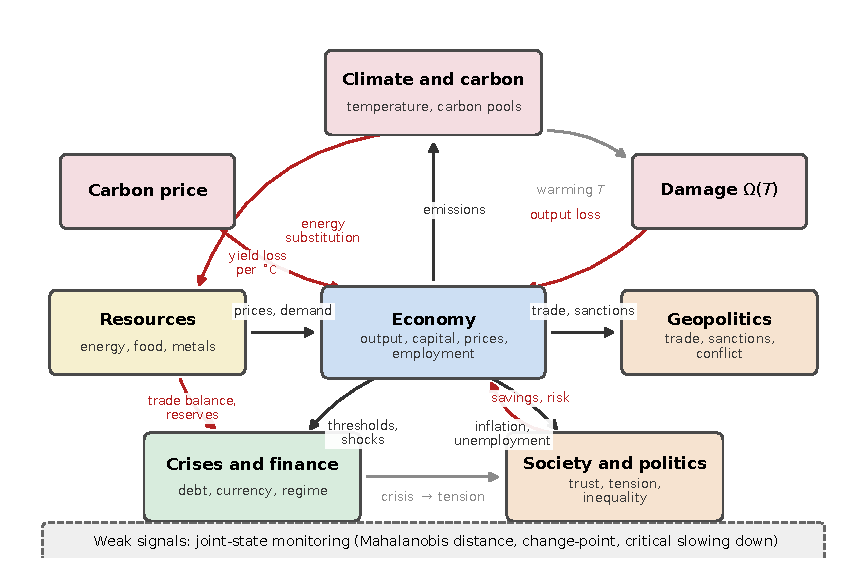
\includegraphics[width=0.98\linewidth]{fig1_architecture.pdf}
\caption{The closed loop. Economy at the hub, physical blocks above it and human blocks below.
Dark arrows are direct effects; red arrows are the channels that reduce output, savings or
supply --- climate damage, energy substitution, the per-degree yield loss on crops, and the
resource trade balance that drives reserves and the sovereign channel. The climate loop
(emissions $\to$ warming $\to$ damage $\to$ output) is complemented by carbon-price, resource,
socio-political, geopolitical and discrete-crisis channels. The bottom layer monitors the joint
state for weak signals.}
\label{fig:arch}
\end{figure}

\subsection{Numerical implementation and the annual algorithm}
\label{sec:arch:numerics}

In a threshold-carrying nonlinear model the update \emph{order} is part of the numerical
specification, not an implementation detail, so we give it in full. Algorithm~\ref{alg:step}
is the effective write order of one call to \texttt{step\_world()} in
\texttt{gim/core/simulation.py}; the same listing is maintained as
\texttt{docs/SIMULATION\_STEP\_ORDER.md} in the archive and is checked by a test.

\begingroup\small
\setlength{\LTcapwidth}{\linewidth}
\begin{xltabular}{\linewidth}{@{}r L >{\raggedright\arraybackslash}p{2.1cm}@{}}
\caption{Algorithm 1: one annual GIM step, $x_{t}\mapsto x_{t+1}$. Steps run once, in this
order, with no intra-year iteration and no market-clearing fixed point; the four-phase
scaffold on the right is the runtime's write-authority contract.}\label{alg:step}\\
\toprule
\# & Operation & Phase \\
\midrule
\endfirsthead
\multicolumn{3}{@{}l}{\emph{Table \thetable{} --- continued}}\\
\toprule
\# & Operation & Phase \\
\midrule
\endhead
\bottomrule
\endlastfoot

1  & refresh relative metrics (shares, ratios, gaps) & baseline \\
2  & update political states; update institutions & baseline \\
3  & generate policies; apply political constraints & baseline \\
4  & resolve foreign policy & detect \\
5  & apply sanctions effects; apply security actions & propagate \\
6  & update active conflicts; apply trade-barrier effects & propagate \\
7  & apply policy actions; apply trade deals; update endogenous relations & propagate \\
8  & allocate energy reserves and caps; update resource stocks & propagate \\
9  & update global resource prices & propagate \\
10 & update global climate (carbon pools, forcing, two-layer heat balance) & propagate \\
11 & update climate risks; apply climate extreme events (off in headline runs) & propagate \\
12 & update economy output (CES, damage, capital) & propagate \\
13 & update public finances (budget, debt, credit cost) & propagate \\
14 & check financial crises: debt trigger, then FX trigger & propagate \\
15 & update inflation and unemployment (Phillips, Okun, energy and food cost-push) & propagate \\
16 & update migration flows; update population & propagate \\
17 & update social state (trust, tension, inequality, legitimacy, protest) & propagate \\
18 & check regime stability & propagate \\
19 & canonical finalisation of critical fields; clamp to declared bounds & reconcile \\
20 & refresh relative metrics; update agent memory; update credit ratings & reconcile \\
21 & $t \leftarrow t+1$ & reconcile \\
\end{xltabular}
\endgroup


\paragraph{Integration and time stepping.} Only the climate block carries continuous-time
dynamics. The four-pool carbon impulse response is integrated exactly over the annual step
($C^{(i)}_{t+1}=C^{(i)}_t e^{-1/\tau_i}+a_i E_t$, Eq.~\ref{eq:pools}), so no discretisation
error enters the carbon stock. The two-layer energy balance (Eq.~\ref{eq:ebm}) is advanced by
explicit Euler at $\Delta t = 1$\,yr. With the headline surface heat capacity
$C_s = 8$\,W\,yr\,m$^{-2}$\,K$^{-1}$ and feedback $\lambda = 1.24$\,W\,m$^{-2}$\,K$^{-1}$ the
stability limit of that scheme is $\Delta t < 2C_s/(\lambda+\kappa) = 7.1$\,yr, so the annual
step is comfortably inside it across the whole prior box: the tightest corner sampled
($C_s = 6$, ECS $=1.5$\,\degC{} giving $\lambda=2.47$, $\kappa=1.3$) still gives a limit of
$3.2$\,yr, and the high-sensitivity corner the reviewer of such a model will ask about
($C_s=18$, ECS $=6$\,\degC) gives $35$\,yr. Accuracy, not stability, is therefore the binding
question, and it is small: re-integrating the baseline forcing path at $\Delta t = 1/12$\,yr
changes the 2100 surface temperature by $0.002$\,\degC{} at the headline parameters and by at
most $0.012$\,\degC{} at any corner of the prior box --- an order of magnitude below the
in-sample temperature RMSE of Section~\ref{sec:valid}. Every other block is a first-order difference equation in annual
time; there is no inner iteration and no convergence criterion to report, because the annual
map is evaluated once rather than solved to a fixed point. Within-year market clearing is
therefore imposed by construction rather than converged to, a consequence
Section~\ref{sec:limits} carries.

\paragraph{Thresholds and discrete events.} Crisis triggers are hard comparisons on state
ratios (Appendix~\ref{app:spec}), so the annual map is piecewise smooth with jump
discontinuities on the trigger manifolds. This matters for the numerical Jacobian of
Section~\ref{sec:stability}: a central-difference stencil that straddles a trigger returns a
meaningless derivative. We therefore verify, at each linearization point, that no trigger
changes state anywhere in the stencil (it does not, at $\varepsilon = 10^{-4}$ of coordinate
scale), and we report the sensitivity of the spectral radius to $\varepsilon$.

\paragraph{Reproducibility and verification.} The engine is deterministic given a seed:
repeated runs of the same configuration are bit-identical on the same platform, and the
regression suite pins golden trajectories that any change to the core must either reproduce to
the bit or explicitly re-baseline with a written reason
(\texttt{scripts/regenerate\_backtest\_baseline.py} refuses to write when a guarded metric
regresses by more than $1\,\%$ without an override flag). The suite carries \nTests{} tests
and \nSubtests{} subtests, including a ten-year 57-agent golden world run and a guard that
every crisis channel fires at least once; it runs in about two minutes on a consumer laptop.
Calibration inputs are checksum-bound and every run writes a manifest recording the code
version, the input digests and the random seeds. Following the ``evaludation'' distinction
\citep{augusiak2014}, we treat this apparatus as \emph{verification} --- evidence that the
implementation computes the intended equations --- and reserve \emph{corroboration} for
Section~\ref{sec:valid}. Cross-platform bit-identity is not claimed: results are reproducible
to floating-point tolerance across platforms and bit-identical within one.

\subsection{Configuration: which mechanisms are active}
\label{sec:arch:config}

GIM ships optional mechanisms as switches, off by default unless anchored by evidence. Because
several of the paper's claims depend on which switches are set, Table~\ref{tab:config} gives
the complete headline configuration and states where each setting is used. Every number in
this paper other than those explicitly marked as ablations was produced with this
configuration.

\begingroup\small
\setlength{\LTcapwidth}{\linewidth}
\begin{xltabular}{\linewidth}{@{}>{\raggedright\arraybackslash}p{4.2cm} c L >{\raggedright\arraybackslash}p{2.6cm}@{}}
\caption{Headline configuration. ``Provenance'' distinguishes empirical calibration against
observations, structural normalisation, and behavioural or numerical regularisation --- three
different epistemic statuses that a single word ``calibrated'' would hide.}\label{tab:config}\\
\toprule
Mechanism & Headline & Where it enters & Provenance \\
\midrule
\endfirsthead
\multicolumn{4}{@{}l}{\emph{Table \thetable{} --- continued}}\\
\toprule
Mechanism & Headline & Where it enters & Provenance \\
\midrule
\endhead
\bottomrule
\endlastfoot

Extreme climate events & off & all deterministic results; on for the seeded ensemble of Sec.~\ref{sec:emergent} & structural \\
Continuous climate$\to$tension term (\texttt{TENSION\_CLIMATE\_SENS}) & off & nowhere; magnitude not identified \citep{hsiang2013,buhaug2014} & tagged, unset \\
Trust-gap effect on tension $\sigma_{\mathrm{tr}}=0.060$ (Eq.~\ref{eq:tension}) & \textbf{on} & all runs, incl.\ the spectra of Fig.~\ref{fig:stability} & empirical (WGI trust persistence) \\
Trust mean-reversion pull $\chi=0.10$\,yr$^{-1}$ (Eq.~\ref{eq:trust}) & \textbf{on} & all runs, incl.\ the spectra of Fig.~\ref{fig:stability} & \emph{numerical regularisation}: weakest value lowering $\rho$ at all three linearization points \\
Reserve-accumulation identity & off & disabling it is a disclosed limitation (Sec.~\ref{sec:limits}) & structural (no nominal FX rate) \\
Growth-damage (Burke-type) TFP channel & off & tail scenarios only \citep{burke2015,burke2023} & tail prior \\
Warming-benefit cap; CH$_4$ feedback & off ($0$) & tail scenarios only & tail prior \\
Model-consistent expectations & off & tested, marginal effect unstable & structural \\
LLM policy agents & off & never in a validated configuration & structural \\
Spatial diffusion (tension $0.05$, climate $0.10$, contagion $0.03$) & \textbf{on} & Sec.~\ref{sec:emergent} ablations & expert prior \\
SSP2 productivity anchor & \textbf{on} & long-horizon baseline; ablated in Sec.~\ref{sec:valid} & scenario input \\
Non-CO$_2$ forcing & exogenous & SSP2-4.5 marker \citep{meinshausen2020} & scenario input \\
\end{xltabular}
\endgroup


Two entries in that table deserve to be named as what they are. The trust mean-reversion pull
was selected as the weakest value that lowers the spectral radius at all three linearization
points --- that is, it was chosen \emph{on the diagnostic that Section~\ref{sec:stability}
then reports}. This is circular if read as evidence that the loop is stable, and we do not
read it that way: the honest statement is that a bounded institutional variable with no
restoring force carries a unit root by construction, that GIM supplies the weakest restoring
force that removes it, and that the spectra we report are those of the resulting map.
Section~\ref{sec:stability} gives the spectra at four settings of that pull, including zero,
so the reader can see exactly how much of the result the choice buys.

\section{What the closed loop does: boundedness, measured}
\label{sec:stability}

Convergence claims are cheap, and we do not make one. This section reports three quantitative
diagnostics and states exactly what each licenses. All runs use the deterministic core in the
configuration of Table~\ref{tab:config}; the harness is
\texttt{scripts/run\_stability\_analysis.py}.

\subsection{Spectrum of the one-year map}

We linearize the annual map $x_{t+1}=F(x_t)$ numerically by central differences around the
baseline trajectory at three points along the run. The coordinates differentiated are seven
variables per agent (output, capital, public debt, unemployment, inflation, trust, tension)
plus nine global coordinates (surface and ocean temperature, four carbon pools, three resource
prices): $57\times7+9=\nStateJac$ in all. Eigenvalues are computed on $D^{-1}JD$ with $D$ the
diagonal of trajectory-mean coordinate scales --- a similarity transform that leaves the
spectrum unchanged and only conditions the eigenvector readout.

\paragraph{What this Jacobian is, and is not.} It is \emph{not} the Jacobian of the full
Markov state. GIM's persistent state registry carries $87$ variable families
(\texttt{docs/state\_registry.csv}), including reserves, bilateral relations, alliances,
sanction counters, resource stocks, credit ratings, population and the crisis-duration
counters. Perturbing one of the \nStateJac{} coordinates advances \emph{all} of them for one
year, but only the \nStateJac{} are read back, with the complementary coordinates held at
their baseline values. What we compute is therefore the Jacobian of the projected map
$P\circ F\circ\iota_{\bar x}$ --- a principal submatrix of the full Jacobian, restricted to
the coordinates that carry the model's stocks and prices. Its spectrum bounds the behaviour of
perturbations confined to that subspace; it does not bound perturbations that excite reserves,
relations or crisis counters directly. We state this as a limitation rather than repair it,
because differentiating the full registry would require a state serialisation the engine does
not currently expose, and we flag it as the first item of future work.

\paragraph{Result.} The spectral radius is $\rho(J)=\rhoA$, $\rhoB$, $\rhoC$ at 2026, 2036 and
2046, over $\nModesA$, $\nModesB$ and $\nModesC$ above-unity modes
(Fig.~\ref{fig:stability}a). Two properties of that spectrum set what a stability claim about
a model of this kind can assert.

The first concerns a large cluster of modes at unit modulus: $45$, $12$ and $24$ eigenvalues
lie inside $[0.999,1.001]$ at the three points, and $94$ or more lie above $0.99$. Part of that
cluster is a specification requirement rather than a result, because a bounded state variable
with no restoring force of its own carries a unit eigenvalue by construction. Institutional
trust is the case in point: bounded in $[0,1]$, its drivers must enter as deviations from a
reference or an agent at entirely ordinary conditions loses trust every year without limit. The
deviation form removes that drift but not the unit root, since a walk without drift still sits
at $|\lambda|=1$; GIM therefore gives trust the weak mean reversion its resource prices already
carry (Table~\ref{tab:config}), and we report the spectrum of the resulting map. The first
carbon pool is the second and physically correct case: with $\tau_1=\infty$ it is a perfect
integrator, $\partial C^{(1)}_{t+1}/\partial C^{(1)}_t = 1$ exactly, so the climate block
\emph{contains a conservative direction by construction}. That is a property of the carbon
cycle, not a defect --- but it makes ``the climate subspace contracts'' false.

The second is the result. Modes above unity remain --- the loop does not contract everywhere
--- but their eigenvector mass sits mainly on \emph{economic} coordinates: public debt
compounding near the effective interest rate, unemployment and inflation carry $0.57$, $0.65$
and $0.78$ of the above-unity loading at the three linearization points, against the social
block's $0.43$, $0.35$ and $0.22$. The climate coordinates carry \emph{none} of the
above-unity mass: across every configuration we examined --- four settings of the trust
mean-reversion pull at three linearization points, twelve spectra in all --- the above-unity
mass on temperature, ocean heat and the carbon pools is $0.00$ to two decimals. The defensible
statement is therefore that \emph{the climate coordinates are non-expanding and carry a
conservative direction}, not that they contract, and that the amplifying directions of this
model at this calibration are socio-fiscal. We report it as a property of this model at this
calibration, not as a general feature of coupled world models.

\paragraph{Sensitivity of the diagnostic.} Two robustness checks belong with the number.
First, the trust mean-reversion pull, which Table~\ref{tab:config} flags as numerical
regularisation: at pull $=0$ the radius is $1.075$, $1.100$, $1.076$ over $75$, $79$, $67$
above-unity modes; at $0.05$, $1.052$, $1.100$, $1.100$ over $50$, $48$, $49$; at the headline
$0.10$, $\rhoA$, $\rhoB$, $\rhoC$ over $38$, $35$, $32$; at $0.20$, $1.020$, $1.100$, $1.100$
over $34$, $29$, $32$. The pull roughly halves the count of above-unity modes and moves the
radius by at most $0.04$; it does not change the qualitative picture, and the climate mass is
$0.00$ at every setting. Second, the differentiation step. Because the map is piecewise
smooth, a central-difference stencil straddling a crisis trigger would return a meaningless
derivative; we verified that no trigger changes state anywhere in the stencil at the headline
$\varepsilon=10^{-4}$ of coordinate scale, and recomputed the whole spectrum at
$\varepsilon\in\{10^{-3},10^{-4},10^{-5}\}$ at the 2026 linearization point. The radius is
$1.03631$ at all three, identical to five decimal places over two orders of magnitude in the
step, and the count of modes above $1.001$ is $32$ at all three. Only the raw count above
$1.000$ moves ($36$, $36$, $37$), because $45$ eigenvalues sit inside $[0.999,1.001]$ and a
handful cross the line under rounding. We therefore quote the radius as a converged result and
the above-unity mode count as an approximate descriptor, and recommend the same caution to
anyone reporting above-unity counts for a model whose spectrum is this dense at the unit
circle.

\subsection{Perturbation contraction}

The trajectory-level counterpart: twin runs from $\varepsilon$-perturbed initial states, gaps
measured as dimensionless relative differences in world product. A $+0.1\,\%$ shock to United
States output --- a vector with essentially no projection on the socio-fiscal modes above ---
produces a relative gap of $2.6\times10^{-4}$ after one year that \emph{contracts} to
$1.2\times10^{-4}$ by year 30, an empirical factor of $0.975$ per year; a $+0.01$\,\degC{}
temperature perturbation decays at $0.970$ per year. Nearby trajectories converge in the
economic--climate subspace --- the opposite of chaotic divergence
(Fig.~\ref{fig:stability}b). The one persistent direction is the one the spectrum names:
raising every country's tension by $0.01$ leaves output almost untouched for a decade and then
amplifies as crisis triggers engage, reaching a $2.5\,\%$ world-product gap by 2053.

The spectrum and the twin runs therefore tell one story: contraction in the
physical--economic directions, slow amplification confined to the socio-fiscal subspace. We
report the asymmetry as a substantive property, not a defect --- and it quantifies the
limitation that socio-political initial-state error does not wash out
(Section~\ref{sec:limits}). Two caveats bound the reading. These are three specific
perturbation directions, not a norm bound: for a non-normal $J$ a full-state perturbation can
be amplified transiently even when every direction we tested contracts, and we have not
computed the finite-time amplification operator $G(t)=\|\delta x(t)\|/\|\delta x(0)\|$ over
random full-state perturbations. And the gap metric is the relative world-product gap, which
is insensitive by construction to directions that redistribute output without changing its
total.

\begin{figure}[!htbp]
\centering
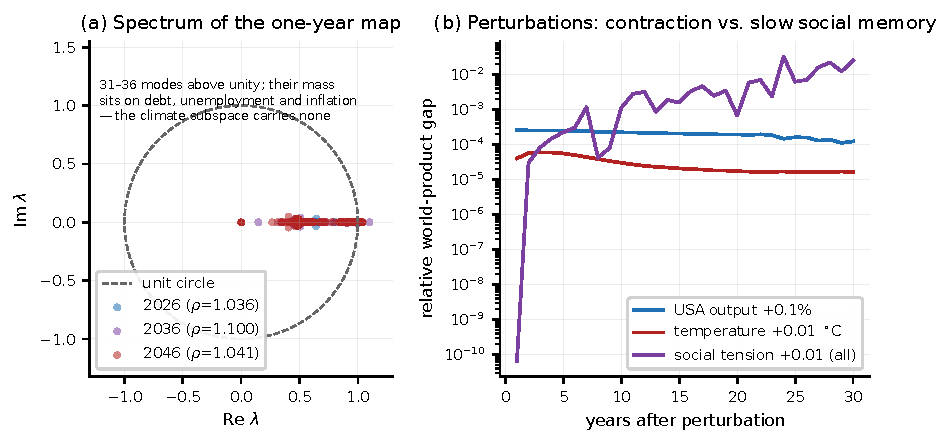
\includegraphics[width=0.98\linewidth]{fig12_stability.pdf}
\caption{Local behaviour of the annual map. \emph{(a)}~Eigenvalues of the (similarity-)
normalized Jacobian of the \nStateJac-dimensional projected state at three linearization
years. The spectrum lies on and inside the unit circle apart from $\nModesC$--$\nModesA$ modes
just outside it, giving $\rho(J)=\rhoA$, $\rhoB$, $\rhoC$; their eigenvector mass sits mainly
on economic coordinates --- public debt, unemployment, inflation --- carrying $0.57$--$0.78$
against the social block's $0.22$--$0.43$, while the climate coordinates carry none of it.
Note the dense cluster at unit modulus: the $\tau=\infty$ carbon pool is a perfect integrator
and contributes $|\lambda|=1$ by construction. \emph{(b)}~Twin-run response (relative
world-product gap): output and temperature perturbations contract at $0.975$ and $0.970$ per
year, while a broad social-tension perturbation persists and amplifies --- the model's one
long-memory direction.}
\label{fig:stability}
\end{figure}

\subsection{Bounded, near-linear growth of parametric spread}

A 500-member ensemble drawing the 33 key parameters from their priors --- with the
discrete-crisis machinery \emph{active} (members average one to three sovereign crisis
episodes by 2053) --- runs the full 30 years without a member diverging or saturating
(Fig.~\ref{fig:ens30}). This is a \emph{parametric, conditional} fan, not a forecast interval. Members share the
initial state, so much of its near-linear growth is each member following its own prior-drawn
trend, and the fan varies $\partial x_t/\partial\theta$ where the twin runs vary $\partial
x_t/\partial x_0$ --- different objects. A parametric fan that does not explode is \emph{not}
independent evidence of dynamical stability: unstable directions may be poorly excited by
parameter perturbations, or invisible in world product. We report it as a bounded parametric
sensitivity and nothing more.

What the fan does bound is the amplification rate: the world-product half-width grows from
$\pm1.7\,\%$ of median at year 5 to $\pm4.0\,\%$ at 10 and $\pm\fanThirty\,\%$ at 30 (all
5--95th half-widths), an average exponential rate below $0.08$\,yr$^{-1}$ with concave shape
after year 10. Two non-trending observables make the point without the trend caveat: the
mean-tension fan stays narrow and sub-linear (5--95th width $0.011$ at year 5, $0.026$ at 30,
i.e.\ $2$--$5\,\%$ of its level), and the temperature fan widens only from $0.72$ to
$1.10$\,\degC{} between years 5 and 30 (full widths; the climate-sensitivity prior expresses
itself early). Median 2053 world product is $\gdpMed$ trillion USD (5--95th:
$\gdpLo$--$\gdpHi$) at $+\tempMed$\,\degC{} ($\tempLo$--$\tempHi$); for calibration of scale, a
single structural choice --- renormalising production to constant returns --- moves 2100 world
product by $7$--$9\,\%$, of the same order as this whole parametric fan.

\paragraph{The ensemble is a prior ensemble, and we say so.} We previously described this fan
as history-matched. It is not, and the diagnostic that would make it so does not bind. The
published configuration runs a single wave of $60$ Latin-style draws over the six
backtest-driving parameters; at the three-sigma implausibility cut the acceptance rate is
$100\,\%$, so the not-ruled-out-yet region coincides with the prior box and the ensemble draws
all $33$ parameters independently from their priors. Over $600$ draws from the box the maximum
implausibility anywhere is $1.69$ against a cut at $3.0$, with a median of $0.665$; the
per-output tolerances are loose by a consistent factor of about five, and world output spans
only $I=0.594$--$0.619$ across the entire box, meaning the window does not identify the
economic parameters at all. The correct description is a \emph{literature-informed,
empirically calibrated and expert-specified prior ensemble with a non-binding history-matching
diagnostic}, and Section~\ref{sec:valid} shows the diagnostic still earns its keep as a
\emph{ranking}. Tighter tolerances and multi-wave refocusing are future work; the current
tolerances are wide because model discrepancy dominates observational error, and we prefer to
publish that than to tighten tolerances until the filter appears to bind.

\begin{figure}[!htbp]
\centering
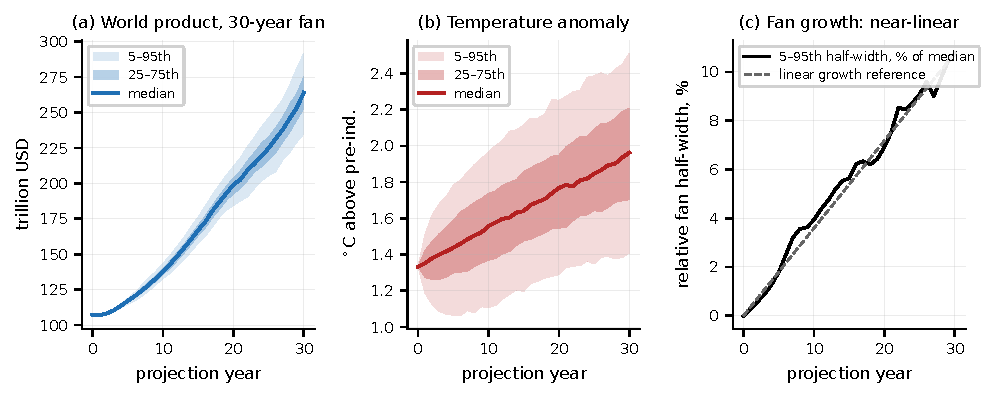
\includegraphics[width=0.98\linewidth]{fig11_ensemble30.pdf}
\caption{Thirty-year boundedness evidence (500-member prior ensemble, shared initial state,
discrete crises active, seed 2026). \emph{(a)}~World product fan: all members bounded, median
$\gdpMed$\,T at 2053, 5--95th $\gdpLo$--$\gdpHi$\,T. \emph{(b)}~Temperature fan: full 5--95th
width grows $0.72\to1.10$\,\degC{} between years 5 and 30, median $\tempMed$\,\degC{} at 2053.
\emph{(c)}~Relative 5--95th half-width of world product reaches $\fanThirty\,\%$ of the median
at thirty years and tracks a linear reference --- parametric spread accumulates, with no
super-exponential bending.}
\label{fig:ens30}
\end{figure}

\paragraph{What ``bounded'' is and is not.} Collecting the three diagnostics: over the tested
thirty-year horizon and the configurations examined, GIM's trajectories are bounded, its
physical and economic perturbations contract, and its parametric spread grows near-linearly,
while a socio-fiscal subspace amplifies slowly and a conservative carbon direction neither
grows nor decays. That is the claim. It is not local asymptotic stability, it is not a
statement about the full Markov state, and it is not a proof --- the evidence is local,
numerical, and specific to this calibration.

\section{Evaluation against observations}
\label{sec:valid}

A bounded simulator can still be stably wrong; the second requirement is anchor to
observation. All retrospective runs are \emph{free-running}: initialized once from the 2015
state and never re-anchored to observations, so errors are multi-year trajectory errors, not
one-step-ahead errors. The output metric is the RMSE over country-year pairs (20 largest
economies) in trillion USD; emissions and temperature are world-series RMSEs against the
Global Carbon Budget \citep{friedlingstein2023} and HadCRUT5.1.0.0 rebased to 1850--1900
\citep{morice2021}. Temperature errors are reported for the deterministic configuration
(internal interannual variability off), which is the configuration every other result in this
paper uses; enabling the variability term raises the in-sample figure from $\rmseTempIn$ to
$\rmseTempInStoch$\,\degC{} because the model's realization is not synchronized with the
observed one, and we give both rather than choosing silently.

The economic and climate blocks are calibrated by history matching --- ruling out parameter
regions whose implausibility $I_o(\theta)=\mathrm{RMSE}_o(\theta)/\mathrm{tol}_o$ exceeds a
three-sigma cut, a standard approach for expensive simulators
\citep{craig1997,williamson2013} --- on the 2015--2023 world series. Predictive adequacy is
then measured by a free-running temporal test on 2020--2023
(\texttt{scripts/run\_holdout\_validation.py}).

\paragraph{How the held-out window is constructed, and what leaks anyway.} The test is
procedurally clean: history matching is re-run with the implausibility computed \emph{only} on
2015--2019, the retained region is frozen, and 2020--2023 is then scored without
re-anchoring. Because the 2015--2019 window rules out no draw at all, the frozen region
coincides with the prior box, and the exercise reduces to running the frozen configuration
forward. That is a real out-of-sample test of the \emph{parameters}. It is not a clean test of
the \emph{model}, and we do not claim it is. Three named channels leak: the structural
decarbonisation rate, the energy elasticity and the TFP sensitivity to R\&D were all set with
reference to the 2015--2023 backtest (Table~\ref{tab:priors1}); the resource-price subsystem
was repaired after comparison with observed 2015--2023 commodity indices; and functional-form
choices throughout the development history were made against the same period. The honest name
for what we report is therefore a \emph{free-running retrospective validation with a
procedurally held-out scoring window}, not an untouched out-of-sample test. Constructing the
latter would require freezing model structure as of 2019 and is not recoverable after the
fact.

\paragraph{That the cut does not bind is itself a result.} History matching here is a
\emph{ranking}, not a filter --- and as a ranking it works: per-output implausibility predicts
its own out-of-sample error at $\rho=0.90$--$0.95$. The usual $\max_o I_o$ aggregation
destroys that information for output ($\rho=+0.06$) because the maximum is almost always taken
by temperature or CO$_2$, whose skill is unrelated to output skill. We report per-output
implausibilities separately for that reason, and suggest others do the same for multi-domain
simulators.

\paragraph{Results.} Table~\ref{tab:backtest} and Fig.~\ref{fig:valid}: in-sample RMSE
$\rmseGdpIn$ trillion USD (country-level output), $\rmseCoTwoIn$ Gt CO$_2$,
$\rmseTempIn$\,\degC; on the held-out 2020--2023 window $\rmseGdpOut$, $\rmseCoTwoOut$ and
$\rmseTempOut$ (with 2020 excluded: $\rmseGdpOutX$, $\rmseCoTwoOutX$, $\rmseTempOutX$). The
per-year decomposition is more informative than the window averages: output errors are $0.56$,
$0.78$, $0.80$, $0.90$ across 2020--2023 --- a monotone free-running drift, not a pandemic
spike, which is why excluding 2020 \emph{raises} the output figure --- while emissions show
the opposite anatomy, a single COVID-sized miss of $1.42$\,Gt in 2020 collapsing to
$0.05$--$0.12$\,Gt in 2021--2023, exactly what a model without a pandemic submodel should
produce when output is nearly right and lockdown-specific emission suppression is outside its
physics; per-year temperature errors are $0.02$--$0.17$\,\degC. Skill against naive benchmarks
built on pre-2020 data divides by output: temperature beats persistence ($+0.05$) and linear
extrapolation ($+0.16$), emissions beat both decisively ($+0.32$, $+0.54$), output loses to
both ($-0.42$, $-3.56$) --- short smooth aggregates remain the domain of a ruler, consistent
with the forecast-evaluation literature \citep{celasun2021}. The climate block additionally
tracks the 1990--2023 record ($0.096$\,\degC) with best-fit sensitivity $3.0$\,\degC,
consistent with the multi-line assessment of \citet{sherwood2020}.

\paragraph{Resource prices are now a validation target, and were not before.} The observed
fixture carried output, emissions and temperature only, so the price subsystem sat outside
every check in the repository. It now carries the World Bank commodity indices
\citep{worldbank_pinksheet} renormalized to the base year, with each tolerance set to the error
a no-skill \emph{flat} price makes, so the implausibility reads directly: below one beats a
flat line. The model scores energy $\priceEnergy$, food $\priceFood$, metals $\priceMetals$.
Adding the check exposed three previously invisible defects --- recycled secondary supply added
on top of a base-year figure that already represented total supply, injecting a permanent
metals glut; a price-damping buffer reading the geological reserve rather than tradeable
inventory, which for energy is fifty years of production in the ground and froze that price at
its initial value for the whole window; and energy demand growing with neither population nor
income. The energy result deserves plain reporting: the model now moves that price in the right
direction but captures only a fraction of the observed amplitude, because the 2015--2023 series
is dominated by the 2020 demand collapse and the 2022 supply shock, neither of which the model
represents. A near-flat energy price is correct for a model without those shocks; what was
wrong before was that it was flat \emph{by construction} rather than by result.

At country level --- where the crisis triggers live --- the 2015--2023 per-country output RMSE
has median $0.10$ and interquartile range $0.05$--$0.13$ trillion USD across the 20 anchored
economies, the largest five errors concentrated where levels are largest (China $2.4$, United
States $1.1$, India $0.27$, Japan $0.24$, United Kingdom $0.17$). Crisis triggers compare debt
and reserves \emph{ratios} within a country, which damps but does not remove the propagation of
level errors into trigger distances --- a caveat carried by the scenario results.

\subsection{Socio-political blocks, including a negative result}

The socio-political blocks are held to a softer but real bar. The conflict-proneness score ---
a fixed-weight composite of observed inputs with no coefficient estimated from conflict data
--- ranks the 57 agents against the UCDP/PRIO Armed Conflict Dataset v24.1 for 1990--2023
\citep{gleditsch2002,davies2024} at AUC $\aucComposite$ (95\,\% CI $[0.60,0.86]$, $20{,}000$
bootstrap resamples \citep{efron1993}; permutation $p\approx0.001$); observed conflict
incidence falls monotonically across score quintiles: $6/11$, $6/11$, $5/11$, $3/11$, $1/13$
countries (55\,\% at the top to 8\,\% at the bottom --- counts this small support ranking, not
calibration, claims).

Chance is the wrong benchmark for a fixed-weight composite, and against the right one the
composite does not survive: its single dominant input, regime stability (construction weight
$0.39$), scores AUC $\aucRegime$ on its own, and the paired bootstrap difference is
$\aucPaired$ with a 95\,\% interval of $[-0.114,+0.031]$ and $P(\text{composite better}) =
0.15$. Social tension alone also edges it ($0.749$). The military term is \emph{below} chance
($\aucMil$) while carrying a $0.20$ construction weight. The blend adds nothing detectable
over one published governance indicator, and a reader wanting a conflict ranking should use
regime stability directly.

We keep the composite in the operational model for a reason worth stating rather than implying:
the static test scores it at base-year values, whereas the model consumes it as a
\emph{dynamic} function of endogenous state --- regime stability, trust, inequality, water
stress and climate risk all move during a run, and the composite is how they reach conflict
risk. Substituting the best static covariate would sever four of those five channels. That is a
design argument, not evidence, and it does not license reporting the composite's AUC as a
success: the negative result is the headline. The Brier skill score against a constant
base-rate forecast is $+0.123$, but the composite is a rank-rescaled index rather than a
calibrated probability, so that figure is a relative statistic between two equally uncalibrated
forecasts.

Because regime stability and military burden are themselves affected by conflict, the score is
recomputed in a vintage-clean configuration (inputs from pre-2000 data only, evaluated against
2000--2023 conflicts): AUC $0.84$ $[0.72,0.94]$, evaluated on the 2000--2023 window and hence
not directly comparable to the 1990--2023 headline, and identical to the 2023-vintage score on
the same subset and window. This shows the ranking is not an artifact of late input vintages.
It does \emph{not} establish absence of reverse causation: pre-2000 regime stability may
itself reflect earlier conflict or a latent common cause, and the test cannot separate those.

The social cost of carbon cross-checks against the published range: Ramsey central
${\approx}\$90$/tCO$_2$ at 200 years, spanning \$90--280 across $(\rho,\eta)$ choices, below
the EPA-2023 central ${\approx}\$190$ \citep{epa2023,rennert2022}. Fed DICE's own damage
function the engine returns ${\approx}\$15$ against DICE's \$31 \citep{nordhaus2018} ---
confirming the higher native estimate is not produced by an inflated valuation layer; the
residual factor of two reflects the 200-year truncation, the different carbon cycle and the
different baseline growth path, and we do not claim a full reconciliation.

\subsection{The long-horizon baseline, and why we do not present it as a projection}

With all headline anchors active, the deterministic baseline reaches $2.75$\,\degC{} in 2100,
with the atmospheric stock rising from ${\approx}3{,}270$ to ${\approx}4{,}470$\,GtCO$_2$
(${\approx}1{,}200$\,GtCO$_2$ of net airborne accumulation, on a preindustrial reference of
$2{,}184$\,GtCO$_2$). Removing the SSP2 productivity anchor --- emissions and decarbonisation
are endogenous either way --- lowers the no-intervention 2100 outcome to about $2$\,\degC. That
this is \emph{nearest} the strong-mitigation SSP1-2.6 envelope is a coincidence of level, not
scenario consistency: GIM's non-CO$_2$ forcing is taken exogenously from the SSP2-4.5 marker
\citep{meinshausen2020} in both cases, so the comparison is a temperature proximity statement
and the construction is a hybrid. The gap between the two is a large, disclosed structural
sensitivity: the structural decarbonisation rate fitted to 2015--2023 ($1.6\,\%$/yr) is
optimistic when extrapolated for decades.

The baseline growth path carries the same warning and we state it in numbers. World product
compounds at $3.06\,\%$/yr to 2053 but at $4.67\,\%$/yr over 2053--2100, reaching
$2{,}256$ trillion USD in 2100. That acceleration is not a projection we defend; it is what
the R\&D and convergence machinery produces when extrapolated three times past its calibration
window, and it is the clearest reason the recommended use mode is scenario \emph{differences}
rather than absolute levels. It also bears on any absolute reading of the game's climate gate
in Section~\ref{sec:instrument}.

\begingroup\small
\setlength{\LTcapwidth}{\linewidth}
\begin{xltabular}{\linewidth}{@{}>{\raggedright\arraybackslash}p{1.9cm} >{\raggedright\arraybackslash}p{2.8cm} L L@{}}
\caption{Evaluation summary. Economic and climate blocks: retrospective evaluation, in-sample
and free-running 2020--2023 (held-out values after semicolons). Other blocks: cross-checks,
benchmark improvement, or channel identification. All values regenerated from release
\Version.}\label{tab:backtest}\\
\toprule
Block & Source & Criterion & Result \\
\midrule
\endfirsthead
\multicolumn{4}{@{}l}{\emph{Table \thetable{} --- continued}}\\
\toprule
Block & Source & Criterion & Result \\
\midrule
\endhead
\bottomrule
\endlastfoot

Economy & PWT \citep{feenstra2015}, WDI \citep{worldbank_wdi} & in-sample country-level RMSE
2015--2023; free-running 2020--2023 & \$\rmseGdpIn\,T; \$\rmseGdpOut{} held out \\
Climate and carbon & AR6 \citep{ipcc_ar6_wg1}, GCB \citep{friedlingstein2023}, HadCRUT5
\citep{morice2021} & in-sample; free-running 2020--2023; ECS/TCR anchors &
CO$_2$ \rmseCoTwoIn\,Gt; \rmseCoTwoOut{} held out. $T$ $\rmseTempIn$\,\degC;
$\rmseTempOut$ held out \\
Resources & World Bank commodity indices \citep{worldbank_pinksheet} & price RMSE vs a
flat-price null (below 1 beats it) & energy \priceEnergy; food \priceFood; metals \priceMetals \\
Cost of carbon & EPA-2023 \citep{epa2023}, RFF-SP \citep{rennert2022} & published cross-check &
\$90 Ramsey central; \$90--280 across $(\rho,\eta)$ \\
Conflict & UCDP/PRIO ACD v24.1 \citep{gleditsch2002,davies2024} & ranking vs.\ registry;
input-vintage test; \emph{best single covariate} & AUC \aucComposite{} $[0.60,0.86]$;
vintage-clean $0.84$ $[0.72,0.94]$; \textbf{but} $1-$regime stability alone \aucRegime,
paired $\Delta{=}\aucPaired$ $[-0.114,+0.031]$ --- the composite adds nothing detectable \\
Social block & SWIID \citep{solt2020}, WGI \citep{kaufmann2011} & \emph{internal} channel
identification on model output (Sec.~\ref{sec:emergent}) & lagged channel identified on the
paired impulse response, not on the level (level vs.\ response $r_s{=}{-}0.33$), $n{=}120$ \\
Boundedness & --- & spectrum; twin runs; fan growth (Sec.~\ref{sec:stability}) &
$\rho{=}\rhoA$--$\rhoB$ over \nModesC--\nModesA{} above-unity modes, above-unity mass economic
($0.57$--$0.78$) with climate mass $0.00$; economic and climate directions contract ($0.975$,
$0.970$/yr); fan ${\pm}\fanThirty\,\%$ at 30\,y \\
\end{xltabular}
\endgroup


\begin{figure}[!htbp]
\centering
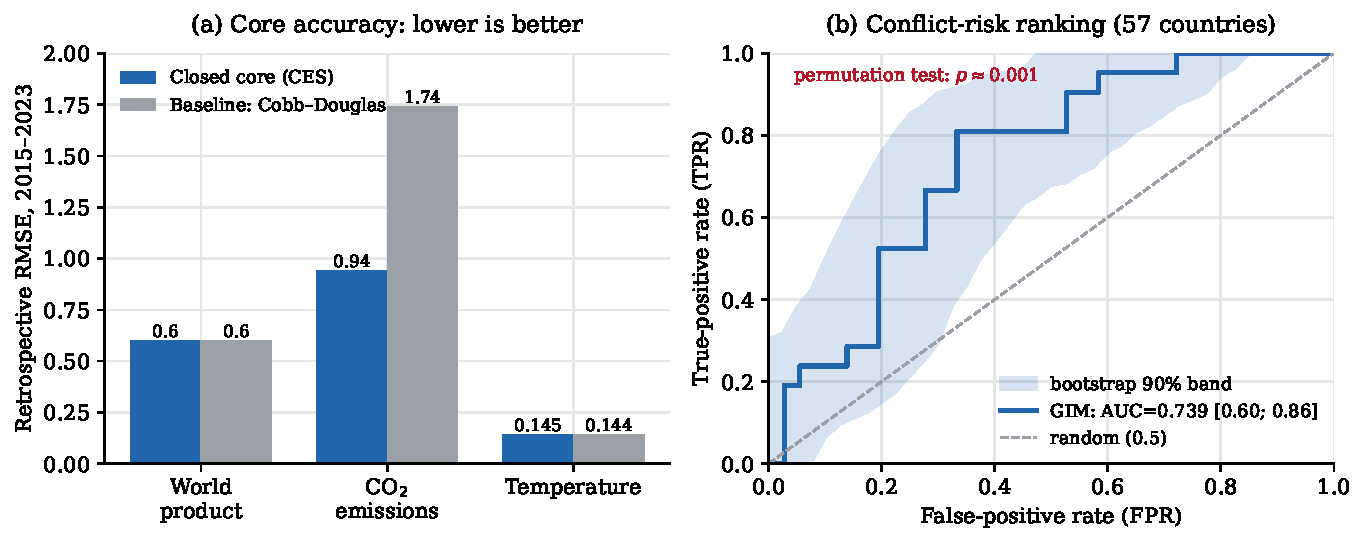
\includegraphics[width=0.98\linewidth]{fig2_validation.pdf}
\caption{Retrospective anchor. \emph{(a)}~In-sample error 2015--2023 in two different units on
one axis, as labelled: world product (trillion USD), emissions (Gt) and temperature (in units
of $0.1$\,\degC, so the plotted $0.99$ is $\rmseTempIn$\,\degC) at left; the three resource
prices at right, scored as the ratio to the error a no-skill flat price makes, so the dashed
line at unity is that null and below it is better. \emph{(b)}~Conflict ranking against the
benchmark that decides it --- not chance, but the composite's own best single input. Bars are
AUC with $95\,\%$ bootstrap intervals; the paired difference and the probability that the
composite is the better ranker are inset (score inputs at 2023 base-year values; the
vintage-clean variant is given in the text).}
\label{fig:valid}
\end{figure}

\section{Cross-domain dynamics}
\label{sec:emergent}

A simulator can be bounded and anchored by being inert. The third requirement is that the loop
produce structured behaviour beyond the coded terms it builds on. We separate three things that
``emergent'' usually conflates: \emph{coded nonlinearity} (a threshold is a threshold),
\emph{cross-domain propagation}, and \emph{endogenously generated ordering and timing}. Only
the third is genuinely a model output rather than a restatement of the code, and we name in
each case which is on offer. Throughout we give effect sizes rather than $p$-values: on
model-generated samples $p$ is a function of the run budget, not evidence about the world. All
causal statements here are \emph{model-internal} --- a paired difference $\Delta y =
y_{\text{shock}}-y_{\text{baseline}}$ identifies the effect of an intervention inside GIM,
which is what a scenario instrument needs and is not a claim about the world.

\paragraph{A lagged economy-to-society channel.} Coded ingredient: linear increments to an
accumulating tension index, whose multi-year timescale follows from accumulation. Which
statistic is used decides the answer, and the point generalises: correlating priors with the
terminal \emph{level} of an accumulating variable recovers whichever coefficients set its
drift, and drift coefficients are coded terms. Only a paired shock-minus-baseline difference
isolates the causal response. Here the two disagree --- level and response correlate at
$r_s=-0.33$ across ensemble members.

Read on the level, tension is led by the base interest rate ($r_s=+0.40$) and equilibrium
climate sensitivity ($r_s=+0.32$), with social priors at $|r_s|\approx0.2$. Read on the
response, a three-year stagflation pulse raises mean tension to a peak of $+0.0031$ five years
later, positive in $76\,\%$ of prior draws, decaying back toward zero by year ten: a hump
rather than a ramp, with transmission confirmed at lag zero and at multi-year lags (cumulative
$+0.33$, within-$R^2$ $0.20$; Fig.~\ref{fig:social}; Morris screening
\citep{morris1991,campolongo2007} alongside). The largest response loading is a climate-damage
parameter ($r_s=-0.35$), while the coded economy-to-society coefficient
\texttt{SOCIAL\_STRESS\_UNEMPLOYMENT\_SENS} is indistinguishable from zero on this statistic
($r_s=+0.13$): the channel reaching society is physico-economic and lagged, and it is not
governed by the parameter whose name says it should be. The spectrum of
Section~\ref{sec:stability} sees the same structure from the other side --- its slow modes load
on trust and tension.

\paragraph{Threshold-stepped sovereign cascades.} The staircase shape is coded. What is not
coded is \emph{which} countries tip, in what order and at what dose: an oil-import burden
propagates through reserves and debt issuance, leaving every importer untouched at
${\leq}3\,\%$ of GDP, tipping three at $6\,\%$, four at $10\,\%$, twelve at $15\,\%$ and
nineteen at $20\,\%$. The ordering is not hand-set, but it is less fiscally determined than we
previously reported. In the headline configuration the Spearman correlations of the tipping
dose against pre-shock debt and reserves are $-0.20$ and $-0.18$, against pre-shock GDP
$-0.38$: country size is the stronger single predictor and the fiscal margins are secondary.
(The $-0.46$ and $-0.44$ quoted in an earlier draft come from a different initialisation than
the tipping counts beside them; mixing the two was an error.) The defensible statement is that
the ordering emerges from pre-shock state rather than a coded sequence, and turns on more than
the debt trigger's own variable --- not that fiscal margins dominate it.

\paragraph{Power-law escalation of food-driven instability.} The social increments are linear
in their inputs (Appendix~\ref{app:spec}), yet protest pressure responds to regional yield loss
as a power law with exponent ${\approx}1.09$ --- consistent in shape with the nonlinearity
reported for food prices and unrest by \citet{lagi2011food} (a working paper; we cite it as
such). Where the curvature originates matters, because composition across a block boundary and
nonlinearity are separate properties. Across a sevenfold dose range the two legs carry similar
exponents ($1.17$ for affordability stress, $1.09$ for protest pressure) and the
protest-to-affordability gain stays inside $0.16$--$0.22$ with no systematic trend: the
resource block generates the curvature and the social block transmits it. Cross-block
composition brings the shock to society; it is not what makes the response nonlinear.

\paragraph{Cross-block synchrony of failures.} On the deterministic 30-year baseline the count
of active crisis states across the 57 agents rises from $\crisisFirst$ per year in the first
decade to $\crisisLast$ in the last. (Two crisis statistics appear in this paper and they are
different objects: \emph{active crisis states} summed over agents and years, as here, and
crisis \emph{episodes} per ensemble member, quoted in Section~\ref{sec:stability} as one to
three sovereign episodes by 2053.) The natural summary of such a rise is a dispersion index,
and it is the wrong one: a Fano index on a trending deterministic series measures the trend, so
comparing it against the homogeneous-Poisson reference of unity tests nothing. Against the
appropriate reference --- an \emph{inhomogeneous} Poisson surrogate carrying the same fitted
intensity, $4{,}000$ draws --- the model shows no excess dispersion at all: surrogate mean
$2.07$ (5--95th $1.43$--$2.78$) against a model value of $1.63$, residual dispersion about a
fitted trend $0.51$. The counts are in fact \emph{more} regular than Poisson. We note this
because dispersion indices are routinely quoted for trending simulated series, where without a
matched-intensity null they are uninformative.

The property that does hold is \emph{synchrony across blocks}. Onsets of economic crises
(sovereign debt, currency; $n=68$) and of social crises (regime; $n=85$) correlate at
$+\syncRaw$ at lag zero. Both series trend, so the raw correlation is confounded, and we give
two detrended versions: after removing a linear trend from each the correlation is $+0.60$,
and on Pearson residuals about a fitted log-linear intensity it is $+0.56$. Detrending
therefore \emph{strengthens} the association rather than explaining it away. Severing every
cross-block channel --- the parameter set is given in the archive --- reduces the lag-zero
correlation to $+\syncAbl$ raw and $+\syncDetAbl$ detrended, i.e.\ by half of its coupled
value in both cases, while the rise in crisis counts falls only from $\crisisLast$ to $12.4$
per year in the last decade. Correlation coefficients do not decompose additively into
attributable shares, so we state the result as measured: removing the coupling halves the
lag-zero correlation and leaves most of the trend intact. The two onset centroids are $2039.5$
and $2043.7$, four years apart --- compatible with a lag-zero peak because the correlation is
computed on annual counts whose year-to-year fluctuations co-move while their slow envelopes
are offset. The ablation is what makes this a measurement rather than an interpretation.

\paragraph{Spatially structured risk.} The diffusion itself is coded (neighbour spillover
weight $0.05$); what is measured is its effect. Switching it on costs under $0.01\,\%$ of the
2015--2023 retrospective fit, and it is not inert: switching the tension channel off raises
the cross-country dispersion of tension by $6.5\,\%$ and quadrupling the weight lowers it by
$2.2\,\%$, monotonically in the weight, while the crisis count moves by up to $21\,\%$ when the
whole spatial layer is removed. The \emph{climate}-risk diffusion, by contrast, has no
measurable downstream effect in the deterministic configuration --- a limit of scope, not a
defect. Climate reaches society only through discrete extreme events, which the deterministic
runs switch off, leaving climate risk with only linear consumers, and a mean-preserving
diffusion of a linear function changes nothing in aggregate. With extreme events enabled over a
12-seed ensemble the same ablation does move tension and crisis counts ($1.7\,\%$ and
$4.3\,\%$). We do not claim the emergent spatial autocorrelation matches the observed record;
that comparison lives in the archive's geographic validation materials.

\begin{figure}[!htbp]
\centering
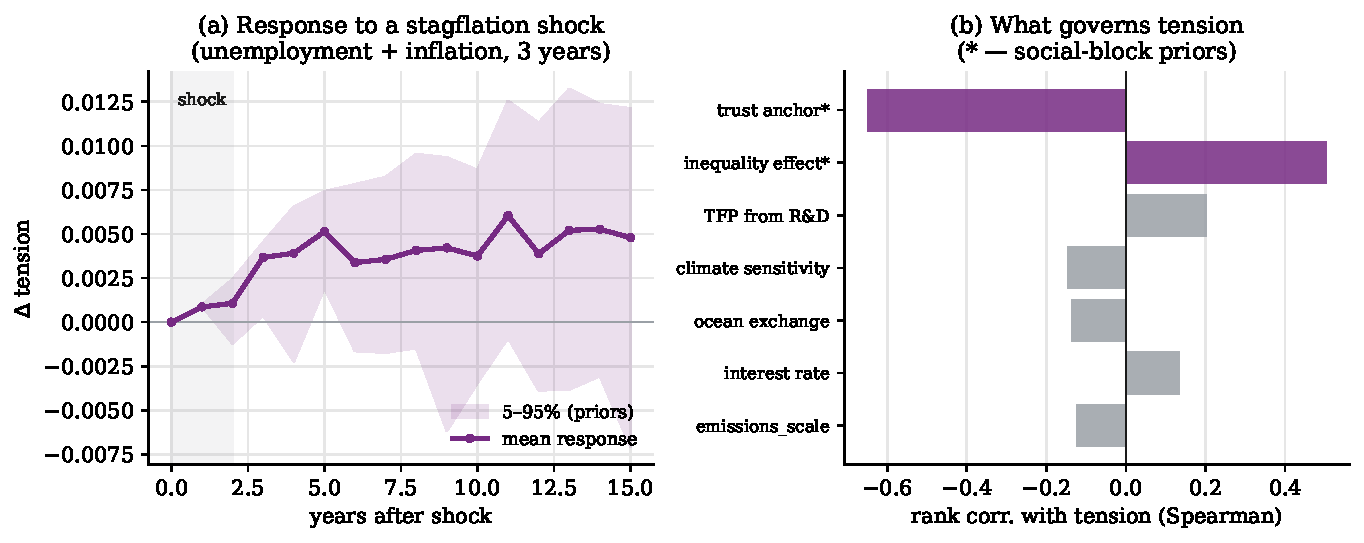
\includegraphics[width=0.98\linewidth]{fig5_social_channel.pdf}
\caption{The economy-to-society channel. \emph{(a)}~Impulse response of mean tension to a
three-year stagflation shock: a hump peaking around year five and decaying by year ten
(5--95th band over priors). \emph{(b)}~What governs tension, contrasting the two questions:
rank correlation of each prior with the final tension \emph{level} and with the causal
\emph{shock response}. Social-block priors are marked~$*$. The level is led by physico-economic
priors, and the two statistics correlate at only $-0.33$ across members, which is why the
claim rests on the paired response in~(a) rather than on the level.}
\label{fig:social}
\end{figure}

\section{The instrument: ensembles, weak signals, and an adversarial tail sampler}
\label{sec:instrument}

The model is operated as an instrument with three modes, in increasing order of
adversarialness.

\subsection{Ensembles and scenario differences}

The core is deterministic, so uncertainty is explicit: 500-member ensembles over the priors
yield outcome distributions, and scenarios are compared as distributions against a common
baseline. The whole workflow runs on a laptop (Apple M4 Pro: a world-year in 30--50\,ms, the
$500\times30$-year ensemble in $109$\,s, the full \nTests-test suite in about two minutes),
which is what makes ensemble-first practice a default rather than a special exercise. A worked
case: a \$50/tCO$_2$ carbon tax cuts emissions by ${\approx}5.5\,\%$ over ten years while
raising tension and lowering trust through the energy-price--inflation channel --- the
political-economy cost invisible to single-domain models, monotone in the rate, and directly
relevant to observed reversals (France 2018, Australia 2014); the full dose--response harness
is Appendix~\ref{app:benchmark}.

We recommend reading GIM in scenario \emph{differences} rather than absolute levels, because
the anchor uncertainties that dominate levels largely cancel between two runs sharing them.
That is a design argument, not a demonstrated result: running one policy scenario across all
500 members and showing that the sign of the difference is stable is the second item of future
work (Section~\ref{sec:limits}), and until it is done the recommendation describes how the
model is built, not how it behaves.

\subsection{Weak signals}

The joint state is monitored for early structure: Mahalanobis distance of the stationary
increments from their recent baseline \citep{mahalanobis1936,wilson1931},
information-criterion change-point detection \citep{schwarz1978}, and critical-slowing-down
indicators \citep{scheffer2009}. An injected $15\,\%$ output drop is flagged at the correct
step while calm runs stay near the false-alarm rate. We report this in one paragraph rather
than as a result: detecting a contemporaneous injected shock is change detection, not early
warning before a transition, and a proper evaluation would need per-detector thresholds,
detection delay, false-positive rate, sensitivity/specificity and a benchmark. We have not done
that; the machinery ships as a monitoring aid and should not be cited as validated
early-warning capability.

\subsection{The game as an adversarial tail sampler}

The same 57-actor core is wrapped into a single-player decision game (GODMODE): annual turns
from 2023 to 2050 (27 turns), 158 dilemma cards compiled into typed policy actions, and seven
catastrophe gates (temperature, biosphere, stability, economic and geopolitical strain, energy
and food prices); losing any gate ends the run, reaching 2050 wins. A game simulates in about a
second, and because players and scripted archetypes push the world into corners smooth history
never visits, the layer functions as \emph{adversarial stress testing} --- targeted exploration
of extreme regions of the state space. We previously called it an importance sampler; that term
is wrong without a proposal density and explicit weights, and we withdraw it. Nothing below is
a probability of a world event: these are frequencies conditional on the selected strategies
and the game's rules, and we report them as a stress-testing method rather than as a third
scientific pillar.

\paragraph{A tail census.} In the 1{,}002-game reference batch, survival is $23.5\,\%$, losses
spread over five causes ($35\,\%$ climate, $22\,\%$ economic, $21\,\%$ geopolitical, $13\,\%$
stability, $8\,\%$ energy price), and $77\,\%$ of failures land in \textbf{2040--2049}
(Fig.~\ref{fig:game}) --- the same clock Section~\ref{sec:emergent} sees in the crisis counts.
Telemetry from the public deployment reproduces that shape with humans in the loop: of 401
runs started, 200 completed, $57$ of them surviving ($28.5\,\%$ of completers, $95\,\%$ CI
${\pm}6.3$ points; $14.2\,\%$ of starts). Under the assumption that runs going badly are
abandoned more often, the completer rate is an upper bound. Human losses spread more broadly
($31\,\%$ climate, $29\,\%$ economic, $15\,\%$ geopolitical, plus biosphere and food-price
tails the bots rarely reach) and $90\,\%$ fall after 2040. This is \emph{not} independent
validation: players drive the same engine, so bot--human agreement shows robustness to how the
strategy space is sampled, not corroboration against observation. No doctrine dominates ---
random play survives most often ($28.4\,\%$) against expansion ($21.9\,\%$) and decarbonisation
($20.1\,\%$), and each dies of its characteristic disease (green of economic strain, $43\,\%$
of its losses; growth of climate and stability, $39\,\%$ and $34\,\%$). Single-axis
optimisation shifting the binding constraint onto another subsystem is the game-mechanical face
of the coupling this paper is about.

\paragraph{A diagnostic that found real defects.} Adversarial play surfaced two symptoms that
no 2015--2023 backtest could show: a resource price that never moved off its clamp, and
government trust falling on hawk and dove paths alike --- an attractor driven by an inequality
drag ${\approx}40\times$ the only restoring term, in the same socio-fiscal subspace the
spectrum of Section~\ref{sec:stability} flags. Diagnosis into root causes came afterwards, from
the price-validation harness of Section~\ref{sec:valid}, which found three separate accounting
and buffer defects behind the pinned prices. Both fixes shipped as equilibrium anchors with the
goldens bit-identical. The epistemic status of the layer is bounded --- no goodness-of-fit
against history, self-selected players, and difficulty gates tuned against the bot batches ---
but it explores exactly the regions that validation against smooth history cannot, and we
regard it as part of the model's quality programme rather than as evidence about the world.

Country policies can also be set by language-model agents (intentions compiled into the same
typed actions, every consequence computed by the deterministic core, off in all validated
configurations, with full audit logs). The whole environment ships as an open, pip-installable
codebase with pinned goldens and manifest-bound runs \citep{theclimateguy2026gim}.

\begin{figure}[!htbp]
\centering
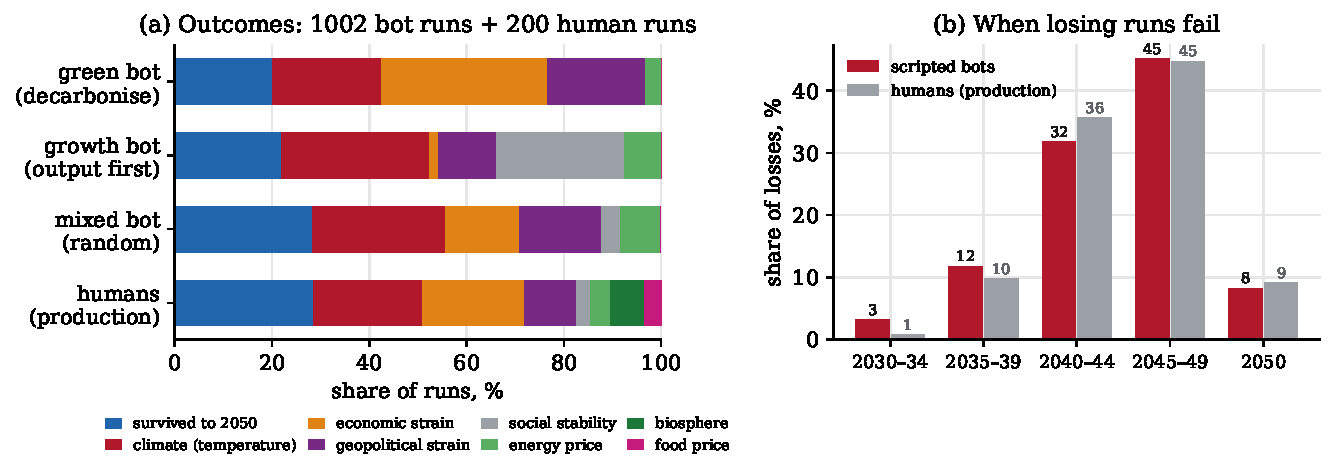
\includegraphics[width=0.98\linewidth]{fig10_game_outcomes.pdf}
\caption{The tail census: 1{,}002 scripted playthroughs and 200 completed human runs (of 401
started; completer statistics shown, an upper bound under the stated attrition assumption),
2023--2050. \emph{(a)}~Outcome composition by archetype and for human players: no doctrine
dominates, each dies of its characteristic cause, and the human loss spectrum is broader
(biosphere and food-price tails the bots rarely hit). \emph{(b)}~Timing of failures, bots vs.\
humans: both distributions peak in 2040--2049 as slow accumulators come due.}
\label{fig:game}
\end{figure}

\section{Limitations}
\label{sec:limits}

\paragraph{Boundedness is engineered and measured, not proven.} The anchors that bound the
loop could mask genuine instabilities of the real system; no formal stability proof for the
full nonlinear map exists, and the evidence of Section~\ref{sec:stability} is local, numerical,
and computed on a \nStateJac-dimensional projection of a larger persistent state. The trust
anchor is the clearest trade-off: without it the model has a unit root in an institutional
variable and the spectral radius reflects that defect rather than the coupling; with it the
model reverts toward each agent's base-year level, which is a non-neutral assumption about the
world over thirty years. Its mean-reversion pull was moreover selected on the very diagnostic
the section reports, and we give the spectra at four settings so the reader can price it.

\paragraph{Structural uncertainty is not represented in the ensembles, and it is large.} The
500-member fan varies parameters. It does not vary structure, initial conditions, or scenario
inputs, and the paper itself contains evidence that structural uncertainty is comparable to or
larger than the parametric kind: removing the SSP2 productivity anchor moves 2100 warming from
$2.75$ to about $2$\,\degC, far outside the parametric fan, and renormalising production to
constant returns moves 2100 world product by $7$--$9\,\%$, of the same order as the entire
30-year parametric spread. A reader should decompose $U_{\text{total}} = U_{\text{parameter}} +
U_{\text{initial state}} + U_{\text{structural}} + U_{\text{scenario}}$ and treat this paper as
quantifying only the first.

\paragraph{The parameter set mixes three provenances} --- literature-grounded, calibrated
against the 2015--2023 backtest, and expert-specified with no external source;
Tables~\ref{tab:priors1} and~\ref{tab:priors2} mark each, and describing all 33 as
``literature-grounded'' would be wrong. Three (the warming-benefit cap, the growth-damage
coefficient and the CH$_4$ feedback) are zero in the headline configuration and sampled only in
tail scenarios, so the headline ensemble varies 30 of the 33 about non-zero centres.

\paragraph{Resource prices reach the economy unevenly.} Forcing each price by a fixed multiple
over a ten-year run moves world output by $-5.5\,\%$ (energy), $-7.9\,\%$ (food) and $+0.8\,\%$
(metals) at a fivefold shock. The metals price is close to inert downstream. Food reaches
society mainly through the trade balance and the sovereign channel rather than through consumer
prices, and the food cost-push term into inflation was added only in this version.

\paragraph{Climate reaches society only through discrete events.} There is no continuous
climate-to-tension term in the headline configuration. One exists in the code, disabled: the
canonical prior for it \citep{hsiang2013} reports a $14\,\%$ rise in intergroup conflict per
standard deviation of warming, but that meta-analysis is contested on sample selection and
analytical coherence \citep{buhaug2014}, with a reply disputing the reanalysis. The direction is
defensible and the magnitude is not identified, so we ship the mechanism off and tagged rather
than choosing a number, and every result in this paper is produced with it disabled.

\paragraph{Crop response to warming is newly endogenous and is not adaptation.} Before this
version warming did not affect crops at all. It now does, at the per-degree yield losses of
\citet{zhao2017} composed with an agricultural supply price elasticity \citep{haile2016};
either alone is misleading, since the yield channel without a supply response drives the food
price to its ceiling. But that supply response is a \emph{price-induced acreage and output
adjustment} --- a market mechanism partly offsetting a yield shock, not climate adaptation,
which would mean crop switching, shifted sowing dates, irrigation, cultivars, relocation and
technology. GIM has none of those, and we withdraw the earlier description of the pair as
supplying adaptation. It gives a $+24\,\%$ food price by 2053, inside the IPCC-assessed range
for climate-driven cereal prices at 2050, an anchor it was not fitted to.

\paragraph{Expectations are adaptive, and long-run growth is weakly identified.} Agents look at
the recent past; a tested model-consistent expectations mechanism is off by default (its
marginal effect proved unstable), so anticipatory responses to announced policy are absent.
Forward projections anchor productivity drift to an external scenario, and the baseline
compounds at $3.06\,\%$/yr to 2053 but $4.67\,\%$/yr thereafter --- an artefact of
extrapolating the R\&D and convergence machinery well past its calibration window, not a
projection. Absolute long-horizon levels inherit this, which is why scenario differences are
the recommended mode.

\paragraph{The climate block is a fast emulator,} not an Earth-system model; the strongest
carbon feedbacks are deeply uncertain, switchable and relegated to tail scenarios. Non-CO$_2$
forcing is exogenous, from the SSP2-4.5 marker \citep{meinshausen2020}: the loop is closed for
CO$_2$ and open for everything else, which qualifies the ``closed loop'' description. The
radiative-forcing coefficient is the \citet{myhre1998} value, not the AR6 update
\citep{forster2021} --- because sensitivity is calibrated at doubling the equilibrium anchor is
unaffected and the transient response is checked directly, but a reader comparing GIM's forcing
to AR6 will find the older constant. Damage estimates are carried as an interval.

\paragraph{The socio-political block mixes anchored and expert-set pieces.} Substantial parts
are tied to literature (war-size tail, migration gravity, misery-index ratio, governance
anchors); coupling thresholds and cross-border tension diffusion remain expert priors, tagged
in the registry. The block supports relative risk ranking (AUC ${\approx}0.74$; vintage-clean
$0.84$) --- and, as Section~\ref{sec:valid} reports, no better than its own strongest input ---
not event prediction. The persistent social mode of Section~\ref{sec:stability} means
socio-political initial-state errors do not wash out, a larger inherited uncertainty than the
economic case.

\paragraph{No nominal exchange rate, and the currency channel depends on that.} The
currency-crisis mechanism fires at a rate and duration consistent with the observed record
($3.5\,\%$ of eligible agent-years against $3$--$5\,\%$ \citep{laeven2020}; mean duration $1.9$
years against $1$--$3$), but only because episode length is bounded explicitly. Nothing rebuilds
reserves, since there is no depreciation to compress imports, so a reserve-accumulation
identity is implemented and deliberately disabled: switching it on drives the crisis rate to
$8\,\%$. Because reserves and debt drive both the sovereign channel and the late-game failures
of Section~\ref{sec:instrument}, the post-2040 rise in active crises and the concentration of
game losses in 2040--2049 may be partly an artefact of this incomplete subsystem; a sensitivity
run with the identity enabled is the third item of future work. Agents that do not issue their
own currency, or that issue a reserve currency, are exempt from the trigger by an explicit
list, because the model has no monetary-union concept and would otherwise flag euro-area
members --- as it did, until the historical backtest caught it.

\paragraph{Aggregation.} Resources are aggregate (no sectoral energy technologies, no
endogenous renewable learning curves); there is no portfolio capital account and no pandemic
submodel (epidemic shocks are extreme events); state-dominated political economies use shared
functional forms with country-specific states; and the annual map is evaluated once, so
within-year equilibration is imposed rather than converged to.

\section{Conclusions}

GIM \Version{} is a closed seven-domain, 57-agent world simulator whose behaviour we measure
rather than assert. (i)~It stays together: a spectral radius of $\rhoA$--$\rhoB$ whose
above-unity modes are mainly economic, whose climate coordinates carry none of the above-unity
mass while containing a conservative direction by construction, with contracting economic and
climate perturbations and near-linear growth of parametric spread over thirty years --- bounded
over the tested horizon, not asymptotically stable. (ii)~It is anchored: in-sample and
free-running held-out retrospective evaluation across output, emissions, temperature and
resource prices, external cost-of-carbon cross-checks, and an input-vintage-robust conflict
ranking reported honestly against its own best single covariate, which it does not beat.
(iii)~It is responsive: a lagged social impulse response, threshold cascades whose ordering is
endogenous, power-law escalation whose curvature we trace to the block that generates it, and
failures that synchronise across blocks more than the blocks alone would produce ---
a synchrony that survives detrending.

Underneath is a stated philosophy: the deterministic core encodes physical conservation laws,
accounting identities and slow empirical regularities with explicit restoring forces, and
parametric uncertainty is carried by ensembles over their strengths. Around it is an
instrument: prior ensembles, weak-signal detectors, and a game layer that adversarially samples
the tails and has already paid for itself by exposing two structural degeneracies no
retrospective test could see. Two of the paper's own diagnostics returned negative results ---
the history-matching filter does not bind, and the conflict composite does not beat its
strongest input --- and we report both rather than removing the tests that produced them.

The model does not forecast; it maps the consequences of assumptions, the distribution of
risks, and the ways a managed world can fail --- comparatively, reproducibly, and on a laptop.

\section*{Code and data availability}

The complete model, calibration data with checksums, every validation and stability harness
cited in the text, the game backend, and the figure-generation scripts are archived as GIM
\Version{} on Zenodo at \url{https://doi.org/10.5281/zenodo.22102520}
\citep{theclimateguy2026gim}. That is the version DOI of the frozen deposit from which every
number in this paper was produced, and it is the record we ask readers to cite; the concept DOI
\url{https://doi.org/10.5281/zenodo.21575176} resolves to whichever version is current and
should be used only when referring to the model in general rather than to these results. The
archive is the citable record; the development repository at
\url{https://github.com/Theclimateguy/GIM} (tag \texttt{v20.1.0}) is a convenience mirror and
is \emph{not} the archival copy. All code and configuration are released under the Apache
License 2.0, an OSI-approved licence. The archive contains the model source; the user manual
and command reference; every configuration file and scenario definition; the pinned observed
fixtures; the pre-processing, run-control and post-processing scripts for every number, table
and figure in this paper; and the \nTests-test regression suite with its golden trajectories.
Reproducing a result is one command per harness, listed in the manual; the figure scripts are
under \texttt{Paper/figures/} and the experiment scripts under \texttt{Paper/revision/scripts/}.

Input and comparison datasets are third-party and are handled as follows.

\begingroup\small
\setlength{\LTcapwidth}{\linewidth}
\begin{xltabular}{\linewidth}{@{}>{\raggedright\arraybackslash}p{3.1cm} >{\raggedright\arraybackslash}p{2.3cm} L L@{}}
\caption{Input and evaluation datasets: version, role and redistribution status. ``Mirrored''
means the file is inside the frozen archive; ``script'' means the archive carries a download
script and a checksum but not the data, because the licence does not permit redistribution.}\label{tab:data}\\
\toprule
Dataset & Version / vintage & Role & Status \\
\midrule
\endfirsthead
\multicolumn{4}{@{}l}{\emph{Table \thetable{} --- continued}}\\
\toprule
Dataset & Version / vintage & Role & Status \\
\midrule
\endhead
\bottomrule
\endlastfoot

World Bank WDI \citep{worldbank_wdi} & 1990--2024 pull, 2026-06 & output, population, debt,
reserves, military expenditure, Gini & CC BY 4.0, mirrored \\
World Bank WGI \citep{kaufmann2011} & 1990--2024, source 57 & regime stability, trust,
legitimacy anchors & CC BY 4.0, mirrored \\
Penn World Table \citep{feenstra2015} & 10.01 & factor shares, depreciation & mirrored \\
Global Carbon Budget \citep{friedlingstein2023} & GCB 2024 workbook, fossil excl.\ carbonation
& emission record and target series & CC BY 4.0, mirrored \\
NOAA GML global mean CO$_2$ \citep{noaa_gml_co2} & global annual mean series, 2024 & base-year
atmospheric stock & public domain, mirrored \\
HadCRUT \citep{morice2021} & 5.1.0.0, rebased to 1850--1900 & temperature target series,
1990--2023 and 2015--2023 & Open Government Licence, mirrored \\
RCMIP non-CO$_2$ forcing \citep{meinshausen2020} & SSP2-4.5 marker & exogenous non-CO$_2$
forcing path & mirrored \\
World Bank Pink Sheet \citep{worldbank_pinksheet} & annual nominal indices, 2010${=}$100,
retrieved 2026-08-24 & resource-price target series & CC BY 4.0, mirrored \\
UCDP/PRIO ACD \citep{gleditsch2002,davies2024} & v24.1 & conflict ranking target &
CC BY 4.0, mirrored \\
SIPRI Military Expenditure \citep{sipri_milex} & 2023 edition & CINC military component &
non-commercial use only --- derived 57-actor aggregate mirrored, source workbook by script \\
SWIID \citep{solt2020} & v9.x & inequality anchor & script \\
Correlates of War NMC & v6.0 & CINC validation & script \\
Hofstede cultural dimensions \citep{hofstede2010} & 2015 release & three dimensions (PDI,
IDV, UAI) enter the tension and trust equations & \textbf{source table not redistributed}: the
scores are not published under an open licence. The public archive carries the ingestion script
and a checksum of the expected input, together with the three-dimension vector for the 57
modelled agents that the engine consumes; the full multi-country source table must be obtained
from the rights holder \\
\end{xltabular}
\endgroup


\section*{Author contributions}

N.S.S.: conceptualization, methodology, software (the simulation engine and the game layer),
investigation, writing --- original draft. A.A.O.: validation (model validation programme),
writing --- original draft and review \& editing. A.N.K.: validation (model and game-simulator
testing), formal analysis (assessment of results), writing --- review \& editing. The archived
software is authored by N.S.S. and A.A.O.; the Zenodo deposit's author list reflects the
software, the byline reflects the paper.

\section*{Competing interests}

N.S.S. and A.A.O. are employees of JSC Sberbank of Russia, whose risk-management activities are
adjacent to the model's stated use cases; the bank had no role in study design, analysis, or the
decision to publish. The authors declare no other competing interests.

\section*{Ethics and player telemetry}

The gameplay telemetry reported in Section~\ref{sec:instrument} contains no personal data. The
public deployment records, per run, only parameters of the run itself: a randomly generated run
identifier, the random seed, the in-game outcome (win/loss, cause, year), the composite score,
and final in-game aggregate metrics. There are no accounts. No names, e-mail addresses, IP
addresses, demographic attributes, device identifiers or any other information that could
identify or be linked to a player is collected, stored or derived at any point; an optional
nickname may be submitted after a run for the public leaderboard and is excluded from the
analysis reported here. Nothing in the collection is personalised, so no individual-level data
exist to report and none are reported. No ethics review was sought, and we state plainly that
none has been obtained rather than asserting that any body has adjudicated the question.

\section*{Financial support}

This research received no funding of any kind and was carried out entirely on the authors' own
time. Article processing charges are borne by the authors.

\section*{Use of generative-AI tools}

Large-language-model tools were used in the preparation of this manuscript. Specifically:
Anthropic Claude and OpenAI GPT models were used (i)~as coding assistants in the development of
the model, its harnesses and its figure scripts; (ii)~to check the internal numerical
consistency of the manuscript against the harness outputs; (iii)~to format and check
bibliographic entries; and (iv)~to review draft text for clarity, grammar and structure, and to
propose rewordings of passages the authors then wrote or rewrote themselves. No section of this
manuscript was generated by a language model and adopted without the authors rewriting it, and
no analysis, result, interpretation or scientific claim was produced by a language model: every
number reported here comes from the deterministic model harnesses named in the text and was
verified by the authors, who take full responsibility for the content. LLM use \emph{inside}
the model is a documented, optional feature (Section~\ref{sec:instrument}) and is off in every
configuration reported in this paper.

\section*{Acknowledgements}

\textbf{TODO: add, or delete this section.} We thank the external players whose anonymous
gameplay produced the telemetry of Section~\ref{sec:instrument}.

\clearpage
\appendix
\renewcommand{\theequation}{A\arabic{equation}}
\renewcommand{\thetable}{A\arabic{table}}
\renewcommand{\thefigure}{A\arabic{figure}}
\setcounter{equation}{0}\setcounter{table}{0}\setcounter{figure}{0}

\section{Model specification}
\label{app:spec}

Symbols follow Algorithm~\ref{alg:step}; agent subscripts are dropped where unambiguous. Every
constant quoted here is the headline value in \texttt{gim/core/calibration\_params.py} of
release \Version{} and is tagged there with its provenance.

\subsection{Production, capital and productivity}

Output is nested CES in capital, labour and energy, normalized to Cobb--Douglas at each
country's base point \citep{arrow1961}:
\begin{equation}
Y = A\,\Theta\,\mathrm{KE}_0^{\,\alpha+\gamma}
    \big(a_K (K/K_0)^{\rho_{KE}} + a_E (E/E_0)^{\rho_{KE}}\big)^{(\alpha+\gamma)/\rho_{KE}}
    L^{\beta},
\qquad \rho_{KE} = \tfrac{\sigma_{KE}-1}{\sigma_{KE}},
\label{eq:ces}
\end{equation}
with $\alpha=0.30$, $\beta=0.60$, $\gamma=0.042$, $a_K=\alpha/(\alpha+\gamma)$,
$a_E=\gamma/(\alpha+\gamma)$, $\mathrm{KE}_0=K_0^{a_K}E_0^{a_E}$. At the base point the inner
aggregator equals one because $a_K+a_E=1$, so levels and first derivatives reproduce the
Cobb--Douglas limit for any $\sigma_{KE}$, while substitution away from it is governed by
$\sigma_{KE}=0.4$ (gross complementarity \citep{vanderwerf2008,koetse2008}; factor shares from
the Penn World Table \citep{feenstra2015,gollin2002}). The exponent sum $0.942$ encodes mild
decreasing returns; per-country scale factors $A$ pin base-year levels, so renormalising to
constant returns moves 2100 world product by $7$--$9\,\%$. $\Theta$ is the climate damage
multiplier of Eq.~\ref{eq:damage}. Capital accumulates as
\begin{equation}
K_{t+1}=(1-\delta)K_t+s_t Y_t,\qquad \delta=0.05,
\label{eq:capital}
\end{equation}
with $s_t \approx 0.24$ modulated by political stability and social tension
\citep{mody2012}. Productivity grows at ${\approx}1\,\%$/yr baseline with an R\&D stock
\'a la \citet{jones1995}, trade-mediated diffusion, and $\beta$-convergence toward the frontier
at slope $0.0093$ per log income gap, validated on the cross-section.

\subsection{Labour market and prices}

Unemployment partially adjusts toward an Okun target \citep{okun1962}:
\begin{equation}
u^{\star}_t = \bar u - \omega\,(g_t - g^{\star}),\qquad
u_{t+1} = u_t + \phi_u\,(u^{\star}_t - u_t),
\label{eq:okun}
\end{equation}
with NAIRU $\bar u = 0.045$, Okun coefficient $\omega=0.30$, potential growth
$g^{\star}=0.025$, adjustment speed $\phi_u=0.5$, and $u$ clamped to $[0.01,0.35]$. Inflation
follows an expectations-augmented flat Phillips curve \citep{phillips1958} with energy and
food cost-push and an optional quantity-theory term:
\begin{equation}
\pi_{t+1} = \underbrace{\theta\pi^{\star}+(1-\theta)\pi_t}_{\pi^{e}}
          + \kappa_\pi(\bar u - u_{t+1})
          + c_E\,\widehat{p}^{\,E}_t + c_F\,\widehat{p}^{\,F}_t
          + \lambda_M\max(0,\widehat{M}_t - g^{\star}-\pi^{\star}),
\label{eq:phillips}
\end{equation}
with anchor weight $\theta=0.5$, target $\pi^{\star}=0.02$, slope $\kappa_\pi=0.25$,
energy pass-through $c_E=0.05$, food pass-through $c_F=0.04$, money pass-through
$\lambda_M=0.027$, hats denoting proportional changes, and $\pi$ clamped to $[-0.02,0.30]$.
Policy rates follow country Taylor rules capped at $\pm6$\,pp \citep{taylor1993}.

\subsection{Public finance, banking and the sovereign channel}

Government budgets close each year: the primary balance plus interest on the debt stock
determines new issuance, the effective interest rate rises with the debt ratio (a financial
accelerator \citep{bernanke1999}), and credit ratings are a function of debt, growth,
inflation and stability. The financial side is stock-flow consistent in the sense of
\citet{godley2007}: within GIM's simplified banking balance sheet each loan creates a matching
deposit and the money stock is identically deposits plus loans; there is no interbank market,
no portfolio choice and no nominal exchange rate. Bilateral trade settles in reserves; world
net exports are demeaned pro rata to GDP so that the world closes to $4\times10^{-18}$ of
world product. Trade volumes follow a gravity law in distance and size
\citep{headmayer2014}.

\subsection{Resources and prices}

Three aggregate resources (energy, food, metals) carry stocks, annual supply, demand and a
world clearing price index normalized to $1.0$ in the base year. Demand grows with population
and income (income elasticity $0.50$ for energy) and responds to price at the market demand
elasticity $0.40$ \citep{labandeira2017}. Supply responds to price and to stock depletion;
food supply additionally responds at the acreage elasticity $0.143$ \citep{haile2016}, and food
yields fall by $4.9\,\%$ per \degC{} of warming \citep{zhao2017}. Each price mean-reverts in
log space toward its reference:
\begin{equation}
\ln p_{t+1} \leftarrow \ln p_{t+1} + \psi\,\big(\ln p^{\mathrm{ref}} - \ln p_{t+1}\big),
\qquad \psi = 0.15\ \text{yr}^{-1}.
\label{eq:priceanchor}
\end{equation}

\subsection{Climate and carbon}

Four-pool AR6 impulse response \citep{joos2013}, integrated exactly over the annual step:
\begin{equation}
C^{(i)}_{t+1} = C^{(i)}_t e^{-1/\tau_i} + a_i E_t,\quad
a=(0.2173,0.2240,0.2824,0.2763),\ \tau=(\infty,394,36.5,4.3)\ \text{yr},
\label{eq:pools}
\end{equation}
with $\sum_i a_i = 1$ exactly (shares rounded here). The atmospheric stock is
$C = C_{\mathrm{pre}} + \sum_i C^{(i)}$ with $C_{\mathrm{pre}}=2184$\,GtCO$_2$; note that
$\tau_1=\infty$ makes the first pool a perfect integrator, which is the conservative direction
Section~\ref{sec:stability} discusses. Forcing is
$F=5.35\ln(C/C_0)+F_{\text{non-CO}_2}$ --- the \citet{myhre1998} coefficient, implying
$F_{2\times}=3.71$\,W\,m$^{-2}$ and, at the calibrated equilibrium sensitivity of $3.0$\,\degC,
a feedback parameter $\lambda=F_{2\times}/\mathrm{ECS}=1.24$\,W\,m$^{-2}$\,K$^{-1}$; the
AR6-updated $F_{2\times}$ is higher \citep{forster2021}, but since sensitivity is calibrated at
doubling the equilibrium anchor is unaffected and the transient response is checked directly
(TCR $1.79$\,\degC, within the AR6 likely range). $F_{\text{non-CO}_2}$ is exogenous, taken
from the SSP2-4.5 marker \citep{meinshausen2020}. Two-layer heat balance
\citep{geoffroy2013}, explicit Euler at $\Delta t=1$\,yr:
\begin{equation}
C_s\dot T = F - \lambda T - \kappa(T-T_d), \qquad C_d\dot T_d = \kappa(T-T_d),
\label{eq:ebm}
\end{equation}
with $C_s=8$, $C_d=100$\,W\,yr\,m$^{-2}$\,K$^{-1}$ and $\kappa=1.0$\,W\,m$^{-2}$\,K$^{-1}$.

Damage enters production as a multiplier, renormalized so that the base year is reproduced
exactly:
\begin{equation}
\Theta(T) \;=\; \frac{1-\zeta T^{2}}{1-\zeta T_{2023}^{2}},\qquad \zeta = 0.0078,
\label{eq:damage}
\end{equation}
so $\Theta(T_{2023})=1$ by construction. The unnormalized function $1-\zeta T^2$ gives
$3.1$, $7.0$ and $12.5\,\%$ losses at $+2$, $+3$ and $+4$\,\degC{} relative to preindustrial,
anchored at the Howard--Sterner productivity-corrected central estimate
\citep{howard2017,nordhaus2017}; a Burke-type growth-damage channel is switchable and off in
the headline configuration \citep{burke2015,burke2023}.

\subsection{Society, politics and discrete crises}

Institutional trust is a $[0,1]$ state driven by deviations, not levels --- the distinction
Section~\ref{sec:stability} explains:
\begin{equation}
\begin{aligned}
\Delta\mathrm{tr}_t = {}& \eta_{y}\frac{y_t - y^{\mathrm{ref}}}{y^{\mathrm{ref}}}
 + \eta_u\,(u_t-\bar u) + \eta_\pi\,(\pi_t-\pi^{\star})
 + \eta_G\,(G_t-G^{\mathrm{ref}})
 + \eta_S\max(0,\,S_t-S^{\mathrm{thr}}),\\
\mathrm{tr}_{t+1} = {}& \mathrm{clip}_{[0,1]}\Big(
   \mathrm{tr}_t+\Delta\mathrm{tr}_t
   + \underbrace{\chi\,(\mathrm{tr}^{\mathrm{anchor}}-\mathrm{tr}_t-\Delta\mathrm{tr}_t)}
     _{\text{mean reversion},\ \chi=0.10\,\mathrm{yr}^{-1}}\Big),
\end{aligned}
\label{eq:trust}
\end{equation}
with $\eta_y=5\times10^{-5}$ per unit of relative income gap, $\eta_u=-0.030$,
$\eta_\pi=-0.015$ (the two-to-one misery-index ratio \citep{ditella2001}), $\eta_G=-0.0004$
per Gini point \citep{wilkinson2009}, $\eta_S=-0.08$ above a tension threshold
$S^{\mathrm{thr}}=0.30$, and $\mathrm{tr}^{\mathrm{anchor}}$ each agent's own base-year WGI
value. Social tension $S\in[0,1]$ accumulates:
\begin{equation}
\begin{aligned}
S_{t+1} = \mathrm{clip}_{[0,1]}\Big(&S_t
 + \underbrace{\sigma_u (u_t-\bar u)+\sigma_\pi(\pi_t-\pi^{\star})}_{\text{economic stress}}
 + \sigma_G (G_t-G^{\mathrm{ref}})\,(1-\mathrm{IDV}/100)\\
 &+ \underbrace{\sigma_{\mathrm{tr}}\,(\mathrm{tr}^{\mathrm{ref}}-\mathrm{tr}_{t+1})}
   _{\text{trust-gap term},\ \sigma_{\mathrm{tr}}=0.060}
 + w_{\mathrm{sp}}\,(\bar S^{\mathcal N}_t - S_t)\Big),
\end{aligned}
\label{eq:tension}
\end{equation}
with $\sigma_u=0.010$ per point of unemployment, $\sigma_\pi=0.005$ per point of inflation,
$\sigma_G=5\times10^{-4}$ damped by the Hofstede individualism score, and a neighbour
spillover $w_{\mathrm{sp}}=0.05$ toward the geographic-neighbourhood mean $\bar S^{\mathcal
N}$. Two distinct mechanisms carry the word ``anchor'' in earlier versions of this paper and we
now name them separately: the \emph{trust mean-reversion pull} $\chi=0.10$\,yr$^{-1}$ in
Eq.~\ref{eq:trust}, and the \emph{trust-gap effect on tension} $\sigma_{\mathrm{tr}}=0.060$ in
Eq.~\ref{eq:tension}. Both are on in every result reported here (Table~\ref{tab:config}).
Legitimacy is $0.6\,\mathrm{tr}+0.4(1-S)$ and sets the policy-space multiplier. Protest
pressure and a food-affordability index are diagnostic composites of tension, inequality and
the food price.

Discrete crises are a state machine with expert-set thresholds, tagged as such in the registry:
\begin{description}\itemsep2pt
\item[Sovereign debt.] Trigger: debt${}>120\,\%$ of GDP \emph{and} effective rate${}>12\,\%$.
  Effect: debt${}\times0.60$ (a $40\,\%$ write-down), output${}\times0.93$, unemployment
  ${}+5$\,pp (capped at $30\,\%$), trust ${}-0.15$, tension ${}+0.15$, stability ${}-0.15$.
  Exit: debt below $70\,\%$ and rate below $8\,\%$, within at most six years.
\item[Currency.] Trigger: external debt${}>50\,\%$ of GDP \emph{and} current-account
  deficit${}>4\,\%$ \emph{and} reserve cover${}<3$ months. Effect: debt${}\times1.10$,
  output${}\times0.85$, unemployment ${}+6$\,pp. Exit: bounded episode length. Agents that do
  not issue their own currency or that issue a reserve currency are exempt by an explicit list
  (Section~\ref{sec:limits}).
\item[Regime collapse.] Trigger: trust${}<0.20$ \emph{and} tension${}>0.80$. Effect:
  output${}\times0.8$, capital${}\times0.7$ \citep{barro2008}. Exit: trust above $0.25$ and
  tension below $0.60$.
\end{description}
Crisis severity is optionally heavy-tailed with a war-size exponent $\alpha_w\approx1.5$
\citep{richardson1948,clauset2009}.

\subsection{Geopolitics, demography and migration}

Interstate relations are a bilateral matrix updated by alliance, sanction, trade and conflict
events; a CINC-style capability index \citep{singer1972} is reconstructed from population,
energy use, output and military expenditure \citep{sipri_milex} and validated against published
CINC values. Population evolves from base birth and death rates ($0.025$, $0.012$/yr) modulated
by income and crisis state; labour supply is a fixed participation share of population.
Migration flows follow a gravity form with income and conflict push terms, capped at a small
share of population per year. A classic Richardson arms-race term was tested and rejected on
the 1995--2024 military-expenditure panel ($p=0.74$) and is not in the model.

\subsection{Prior specification, history matching and ensemble formation}

Priors are per-parameter triangular (30 of 33), lognormal (2) or normal (1) over the ranges of
Tables~\ref{tab:priors1}--\ref{tab:priors2}; the full registry of 287 parameters with
calibration-status tags is in the archive. Implausibility uses tolerances
$\mathrm{tol}_o$ of $6$ trillion USD (world product), $2$\,Gt (emissions) and $0.15$\,\degC{}
(temperature) --- observational uncertainty bundled with an explicit model-discrepancy
allowance --- with the cut $\max_o I_o \le 3$. Resource-price tolerances are set instead to the
error a flat price makes, so an implausibility below one beats the null. The published
configuration uses a single wave of $60$ Latin-style random draws over the six
backtest-driving parameters; at the three-sigma cut the acceptance rate is $100\,\%$, so the
not-ruled-out-yet region coincides with the prior box and ensembles draw all $33$ parameters
independently from their priors (Section~\ref{sec:stability}).

\begingroup\small
\setlength{\LTcapwidth}{\linewidth}
\begin{xltabular}{\linewidth}{@{}>{\raggedright\arraybackslash}p{5.2cm}ccc L@{}}
\caption{Key priors, part 1: the 19 parameters discussed in the text (units inline;
dimensionless unless stated). ``Provenance'' is L = literature, B = calibrated against the
2015--2023 backtest, E = expert-specified, N = numerical regularisation --- the three-way
distinction Section~\ref{sec:limits} insists on.}\label{tab:priors1}\\
\toprule
Parameter & Central & Range & Prov. & Source \\
\midrule
\endfirsthead
\multicolumn{5}{@{}l}{\emph{Table \thetable{} --- continued}}\\
\toprule
Parameter & Central & Range & Prov. & Source \\
\midrule
\endhead
\bottomrule
\endlastfoot

Equilibrium climate sensitivity, \degC & 3.0 & 1.5--6.0 & L & \citep{ipcc_ar6_wg1,otto2013,sherwood2020} \\
Surface heat capacity, W\,yr\,m$^{-2}$K$^{-1}$ & 8.0 & 6.0--18.0 & L/B & \citep{geoffroy2013} \\
Ocean heat exchange, W\,m$^{-2}$K$^{-1}$ & 1.0 & 0.4--1.3 & L/B & \citep{geoffroy2013} \\
Emissions scale & 0.98 & 0.90--1.05 & L & \citep{friedlingstein2023} \\
Structural decarbonization rate, yr$^{-1}$ & 0.016 & 0.010--0.030 & B & GCP/WDI trend \citep{friedlingstein2023}; 2015--2023 backtest \\
Capital share $\alpha$ & 0.30 & 0.22--0.40 & L & \citep{feenstra2015,gollin2002} \\
Labor share $\beta$ & 0.60 & 0.50--0.72 & L & \citep{feenstra2015,gollin2002} \\
Energy elasticity $\gamma$ & 0.042 & 0.015--0.080 & B & 2015--2023 backtest \\
Capital--energy substitution $\sigma_{KE}$ & 0.40 & 0.20--0.60 & L & \citep{vanderwerf2008,koetse2008} \\
Depreciation rate $\delta$, yr$^{-1}$ & 0.05 & 0.03--0.08 & L & \citep{feenstra2015} \\
TFP sensitivity to R\&D & 0.30 & 0.10--0.60 & B & calibration to backtest \\
Damage coefficient $\zeta$ & 0.0078 & 0.0015--0.025 & L & \citep{howard2017,nordhaus2017,burke2015} \\
Pure time preference & 0.015 & 0.001--0.030 & L & \citep{nordhaus2017,stern2007} \\
Elasticity of marginal utility $\eta$ & 1.45 & 1.0--2.0 & L & \citep{nordhaus2017,stern2007} \\
Market demand elasticity & 0.40 & 0.20--0.70 & L & \citep{labandeira2017} \\
\midrule
\multicolumn{5}{@{}l}{\emph{Social block (validated by sign and channel, Sec.~\ref{sec:emergent})}}\\
Tension stress from unemployment $\sigma_u$ & 0.010 & 0.007--0.014 & L/E & \citep{ditella2001}; structural prior \\
Tension stress from inflation $\sigma_\pi$ & 0.005 & 0.003--0.007 & L & \citep{ditella2001}, aversion ${\approx}2{:}1$ \\
Inequality effect on tension $\sigma_G$ & 0.0005 & 0.0003--0.0007 & L/E & \citep{wilkinson2009} \\
Trust-gap effect on tension $\sigma_{\mathrm{tr}}$ (Eq.~\ref{eq:tension}) & 0.060 & 0.039--0.081 & B & calibrated to WGI trust persistence \\
Trust mean-reversion pull $\chi$, yr$^{-1}$ (Eq.~\ref{eq:trust}) & 0.10 & 0--0.20 & \textbf{N} & weakest value lowering $\rho$ at all three linearization points (Sec.~\ref{sec:stability}) \\
\midrule
\multicolumn{5}{@{}l}{\emph{Resource block}}\\
Energy demand income elasticity & 0.50 & 0.33--0.60 & B & IEA intensity trend vs.\ world GDP growth \\
Food yield loss per \degC & 0.049 & 0.031--0.074 & L & \citep{zhao2017}, four independent method families \\
Food supply price elasticity & 0.143 & 0.045--0.79 & L & \citep{haile2016}, aggregate long-run growing area \\
Food price pass-through to CPI $c_F$ & 0.04 & 0.02--0.08 & L & CPI food weight $\times$ commodity-to-retail pass-through \\
\end{xltabular}
\endgroup


\begingroup\small
\setlength{\LTcapwidth}{\linewidth}
\begin{xltabular}{\linewidth}{@{}>{\raggedright\arraybackslash}p{4.0cm}ccc>{\raggedright\arraybackslash}p{1.6cm}L@{}}
\caption{Key priors, part 2: the remaining 14 of the 33 sampled parameters. ``Headline''
records whether the parameter is sampled about a non-zero centre in the 500-member headline
ensemble or is fixed at zero there and sampled only in tail scenarios --- the distinction
Section~\ref{sec:limits} makes explicit.}\label{tab:priors2}\\
\toprule
Parameter & Central & Range & Prov. & Headline & Source \\
\midrule
\endfirsthead
\multicolumn{6}{@{}l}{\emph{Table \thetable{} --- continued}}\\
\toprule
Parameter & Central & Range & Prov. & Headline & Source \\
\midrule
\endhead
\bottomrule
\endlastfoot

Warming-benefit cap & 0 & 0--0.02 & E & tails only & prior (CO$_2$ fertilisation) \\
Warming-benefit peak, \degC & 0.3 & 0--1.0 & E & inactive & deprecated while the cap is 0 \\
Damage risk adjustment & 0.005 & 0--0.02 & E & sampled & prior \\
Deep-ocean heat capacity & 100 & 40--200 & L & sampled & \citep{geoffroy2013}; DICE-2016 \citep{nordhaus2018} \\
Land-use CO$_2$, Gt/yr & 0.6 & 0--1.5 & L & sampled & \citep{friedlingstein2023} \\
Carbon feedback, GtCO$_2$/\degC & 1.5 & 0--5.0 & L & sampled & AR6 WG1 Ch.5 \citep{ipcc_ar6_wg1}; permafrost literature \\
CH$_4$ feedback, W\,m$^{-2}$/\degC & 0.03 & 0--0.1 & L & \textbf{0 in headline} & AR6 WG1 Ch.5 \citep{ipcc_ar6_wg1} \\
Base birth rate & 0.025 & 0.015--0.035 & L & sampled & \citep{worldbank_wdi} \\
Base death rate & 0.012 & 0.007--0.017 & L & sampled & \citep{worldbank_wdi} \\
Neutral interest rate & 0.02 & 0.005--0.04 & L & sampled & IMF WEO; $r^*$ literature \\
Growth-damage TFP coefficient & 0 & 0--0.001 & L & \textbf{0 in headline} & \citep{burke2015} \\
War-size tail exponent $\alpha_w$ & 1.5 & 1.3--1.8 & L & sampled & \citep{richardson1948,clauset2009} \\
Migration base / max share & 0.001/0.003 & see registry & E & sampled & UN DESA; UNHCR \\
Regime-collapse output/capital mult. & 0.8/0.7 & 0.7--0.9 / 0.55--0.85 & L & sampled & \citep{barro2008} \\
\end{xltabular}
\endgroup


\renewcommand{\theequation}{B\arabic{equation}}
\renewcommand{\thetable}{B\arabic{table}}
\renewcommand{\thefigure}{B\arabic{figure}}
\setcounter{equation}{0}\setcounter{table}{0}\setcounter{figure}{0}

\section{Characterisation of cross-sector transfer functions}
\label{app:benchmark}

For three shocks we take a published conclusion from a sectoral model where one exists, feed
GIM the same exogenous shock, and ask whether it (a)~reproduces the sectoral first-order effect
and (b)~exhibits a cross-sector consequence the sectoral model cannot represent by
construction. Runs are deterministic (57 countries, ten years, extreme events off) and each
scenario carries a dose--response sweep. We have retitled this appendix: an earlier version
promised a ``benchmark against a named sectoral model'' in all three cases and delivered a
named model in one. What it actually establishes is the \emph{shape and gain} of three
cross-sector transfer functions, and that is how we report it. Reporting a nonzero GIM slope
against a sectoral anchor's flat one would not be a measurement in any case: a model without a
society block has zero slope on the society axis by construction.

\paragraph{Carbon tax (sectoral anchor: DICE-2016R \citep{nordhaus2017,nordhaus2018}).} Fed the
same \$50/tCO$_2$ tax, GIM reproduces the emissions decline (${\approx}5.5\,\%$ over ten years;
log--log exponent $0.88$ in the tax rate, $R^2=0.999$ over the sweep --- mildly saturating) and
adds the political-economy channel absent from DICE: tension rises and trust falls in the rate,
with exponent $1.82$ ($R^2=0.97$). This is the one case where a published sectoral number is
directly comparable: DICE's optimal carbon price of ${\approx}\$31$/tCO$_2$ (2015, rising
${\approx}3\,\%$/yr) is the anchor for the tax level, and the emissions response is the
first-order effect both models share.

\paragraph{Oil shock (no named sectoral anchor).} An oil-import burden propagates into
sovereign finance through reserves and debt issuance. The response is threshold-stepped: no
importer tips at $3\,\%$ of GDP per year, three tip at $6\,\%$, four at $10\,\%$, twelve at
$15\,\%$ and nineteen at $20\,\%$ (Sri Lanka 2022 is the real-world instance of the mechanism).
Two features of the construction bear stating and both weaken the experiment. First, the supply
cut is converted into an import bill \emph{outside} the model, using an assumed price elasticity
($0.30$) and import intensity ($0.05$) hard-coded in the benchmark harness, and injected
directly into public debt and FX reserves. The scenario therefore exercises the
finance-to-sovereign-crisis leg and does \emph{not} test the resources-to-finance coupling
inside GIM. Second, we cite no published sectoral conclusion here: ``energy-system models''
is not a named anchor, and we do not claim one.

\paragraph{Crop shock (assessment anchor: AgMIP/AR6 range).} A regional yield loss raises
food-affordability stress and protest pressure as power laws of similar exponent ($1.17$ and
$1.09$, $R^2 = 0.997$ and $0.976$) \citep{lagi2011food}: the curvature is generated in the
resource block and transmitted to society, with the protest-to-affordability gain staying
inside $0.16$--$0.22$ across a sevenfold dose range. The assessment chain stops at the
food-security index.

The three channels take distinct forms --- power-law, threshold-stepped, and power-law with a
different exponent (Fig.~\ref{fig:bench-summary}) --- and that variety, rather than a nonzero
slope, is what the exercise establishes.

\begin{figure}[!htbp]
\centering
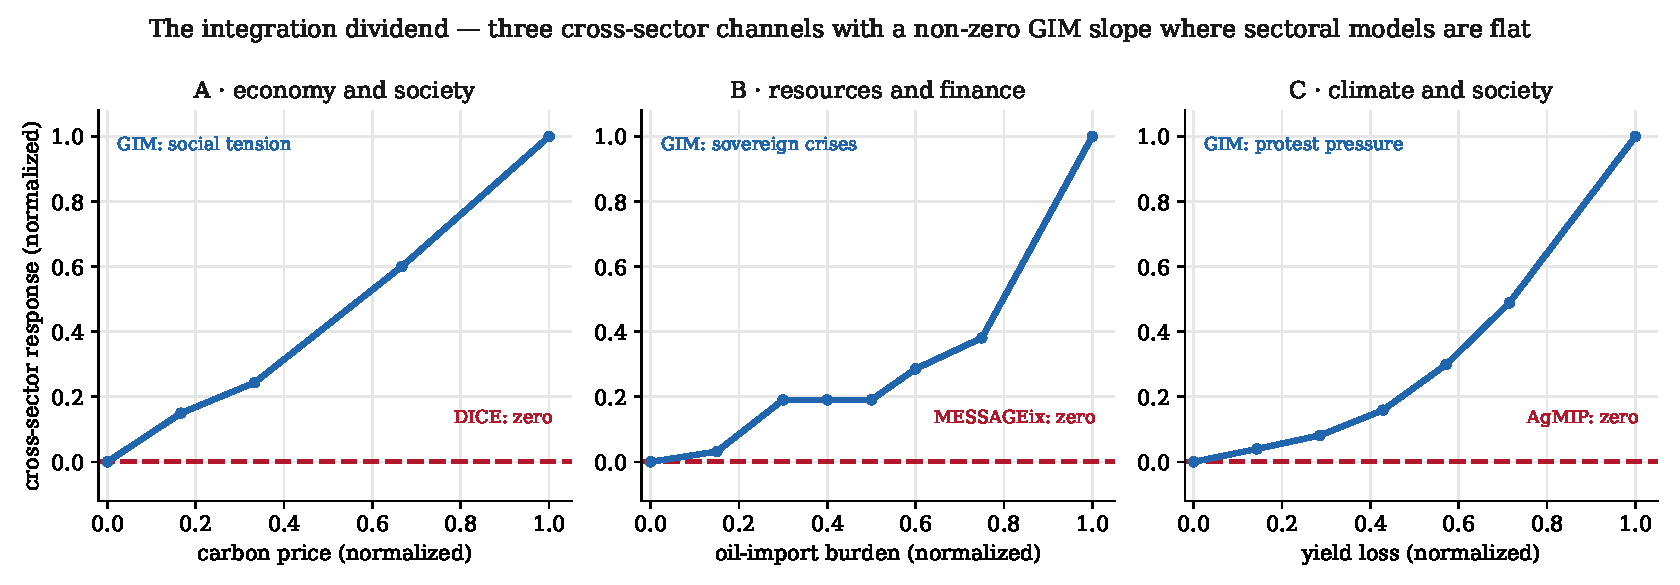
\includegraphics[width=0.98\linewidth]{fig9_integration_summary.pdf}
\caption{Three cross-sector transfer functions, each in its own units.
\emph{(a)}~Carbon price to social tension: a power law, exponent $1.82$.
\emph{(b)}~Oil-import burden to the count of importers entering sovereign debt crisis:
threshold-stepped, six distinct levels, no importer tipping below $6\,\%$ of GDP per year.
\emph{(c)}~Regional yield loss to food affordability (grey) and protest pressure (green):
power laws of similar exponent, $1.17$ and $1.09$, so the curvature is generated in the
resource block and transmitted rather than compounded. Note that the panel's input is an
exogenous \emph{yield} loss, not a temperature change: this is a resources-to-society channel.
A climate-to-society pathway would have to run
$\Delta T \to \Delta Y_{\text{crop}} \to p_{\text{food}} \to$ affordability $\to$ protest, and
GIM now contains every link of that chain (Section~\ref{sec:limits}), but the sweep plotted
here enters at the second link so that the dose is controlled.}
\label{fig:bench-summary}
\end{figure}

\clearpage
\bibliography{references}

\end{document}
